\documentclass[11pt,a4paper]{article}

\usepackage{latexsym}
\usepackage[main=ngerman,english]{babel}
\usepackage[utf8]{inputenc}
\usepackage{amsmath}
\usepackage{graphicx}
\usepackage[colorinlistoftodos]{todonotes}
\usepackage{natbib}
\usepackage{multirow}
\usepackage{url}
\usepackage{microtype}
\usepackage{paralist}
\usepackage{tabularx}
\usepackage{booktabs}
\usepackage{covington}
\usepackage{verbatim}
\usepackage{amsmath}
\usepackage{csquotes}
\usepackage{algorithm}
\usepackage{algorithmic}
\usepackage[skip=4pt]{caption}
\usepackage[nohyperref]{acl2018}
\usepackage[ngerman]{hyperref}
\usepackage{xcolor}
\usepackage{rotating}
\usepackage{afterpage}
\usepackage{pdflscape}

\newcommand{\lang}[1]{\textit{#1}}
\newcommand{\action}[1]{\texttt{#1}}
\newcommand{\prostst}[0]{\emph{CoNLL--SIGMORPHON 2018 Shared Task}}

\newcommand{\algorithmautorefname}{Algorithmus}

% Geklaut aus der hyperref-Integration von acl2018.sty
% Ich kann nicht auf deren Implementation zurückgreifen, weil \autoref sonst die falsche Sprache (Englisch) wählt
\definecolor{darkblue}{rgb}{0, 0, 0.5}
\hypersetup{colorlinks=true,citecolor=darkblue, linkcolor=darkblue, urlcolor=darkblue}

\aclfinalcopy

\title{Projektbericht Sprachtechnologie 2018}

\author{
Fynn Schröder\\
(7003971)
\\\And Marcel Kamlot\\
(6208685)
\\\And Gregor Billing\\
(6808038)}

\date{20.09.2018}

\begin{document}
\maketitle
\pagestyle{plain}
\pagenumbering{arabic}

\begin{abstract}
Im Projekt \textit{Sprachtechnologie} haben wir den \prostst~mit dem Title \enquote{Universal Morphological Reinflection} bearbeitet. Unser Arbeitsergebnis ist ein neuronales Netzwerk in Anlehnung an \citet{cluzh:MakarovRC17}, das wir um mehrere Kernfunktionen ergänzt haben. Hervorzuheben ist dabei die Einbindung von grafischen Features noch unterhalb der Zeichen-Ebene, die wir in mehreren Konfigurationen auswerten und sprachübergreifend vergleichen. Als Erkenntnis kristallisiert sich heraus, dass diese Zusatzinformationen auf einigen Sprachen helfen, auf anderen jedoch keinen Mehrwert liefern. Eine weitere Verbesserung der Ergebnisse erzielen wir überdies durch den Einsatz von \textit{Beam-Decoding} und der künstlichen Erweiterung der Trainingsdaten.
\end{abstract}

\section{Einleitung und Aufgabenstellung}
\label{sec:introduction}
In diesem Projekt haben wir uns mit Flexion, also dem morphologischen Prozess der Wortbildung durch Anpassung an die grammatische Funktion innerhalb des Satzes, befasst. Im Deutschen bezeichnet dies üblicherweise die Deklination von Substantiven und Adjektiven nach Kasus, Numerus und Genus sowie die Konjugation von Verben.
Andere Sprachen unterliegen jedoch unterschiedlichen Flexionsparadigmen, und somit wurde von Anfang an darauf geachtet, ein möglichst sprach-unabhängiges System zu entwerfen das in der Lage ist, die tatsächlichen Strukturen einer Vielzahl von Sprachen zu lernen und anwenden zu können.

\subsection{SIGMORPHON Shared Task}
\label{sec:sub:shared_task}
Die Arbeit entstand als Teil des \textit{CoNLL--SIGMORPHON 2018 Shared Task} von \citet{sigmorphon:st2018}. Er besteht aus zwei Aufgaben: Für Aufgabe 1 wurden gemäß des \textit{UniMorph}-Standards \citep{kirov:unimorph2018} annotierte Daten in über 100 Sprachen veröffentlicht. Diese Datensätze sind dabei jeweils in bis zu drei verschieden Größenordnungen verfügbar, siehe \autoref{fig:training-volumes}. Sie bestehen pro Beispiel aus je einer Grundform (\textit{Lemma}), der flektierten Form (\textit{Flexion}) sowie den Eigenschaften (\textit{Features}) der flektierten Form; in \autoref{fig:german-declension} sind deutsche Beispiele dargestellt. Aufgabe ist es, aus einem gegebenen Lemma und einer dazugehörigen Menge an Features die flektierte Vollform zu generieren.

\begin{table}[htb]
\centering
\begin{tabular}{lrr}
\toprule
%& \multicolumn{2}{c}{Anzahl Trainingsexemplare}\\ \cmidrule{2-3}
Bezeichnung & Maximum & Durchschnitt\\
\midrule
low & 100 & 99.6\\
medium & 1.000 & 934.5\\
high & 10.000 & 8553.6\\
\bottomrule
\end{tabular}
\caption{Anzahl der Trainingspaare je Datensatz}
\label{fig:training-volumes}
\end{table}

\begin{table}[htb]
\centering
\begin{tabular}{llr}
\toprule
Lemma & Flexion & Features\\
\midrule
Baumhaus & Baumhäuser & N;ACC;PL\\
Vogel & Vögeln & N;DAT;PL\\
Milchkuh & Milchkühen & N;DAT;PL\\
\bottomrule
\end{tabular}
\caption{Beispiel-Tupel aus dem Trainingsdatensatz \lang{german}}
\label{fig:german-declension}
\end{table}

Erst kurz vor Ende der Entwicklungszeit wurde dann ein Test-Set veröffentlicht, auf dem es gilt eine möglichst hohe Accuracy zu erreichen.
Wir haben es uns darüber hinaus als Ziel gesetzt, die Levenshtein-Distanz der Ausgabe zu minimieren. Es wurden zur offiziellen Bewertung der Qualität der Ergebnisse nämlich zwei verschiedene Metriken angewandt:
\begin{itemize}
    \item \textbf{Accuracy} als Standardmaß von korrekten Ausgaben im Verhältnis zu allen Ausgaben des Systems insgesamt
    \item \textbf{Levenshtein-Distanz} gemäß der klassischen Definition von \citet{levenshtein:binary66} um festzustellen, wie weit eine Ausgabe des Systems vom Goldstandard entfernt liegt. Insbesondere hat eine korrekte Ausgabe des Systems also immer einen Distanz-Wert von $0.0$
\end{itemize}
Ebenso wurde zusammen mit den Trainingsdaten ein Baseline-System ausgeliefert, das als Richtwert dient. Wir haben es uns zum Ziel genommen, in möglichst vielen Sprachen mit den Accuracy-Werten möglichst weit über den Ergebnissen dieses Baseline-Systems zu liegen.
Dieses Baseline-System wird in \autoref{sec:baseline} näher erläutert.

Letzten Endes wurden alle Systeme der Teilnehmer nach ihrer Accuracy miteinander verglichen, und wir haben uns dabei mit unserer Abgabe im oberen Mittelfeld positioniert. Insbesondere haben wir unsere Zielsetzung weitestgehend erreicht, und bis auf vereinzelte Ausreißer (die unter \autoref{sec:results} noch diskutiert werden) die Werte der Baseline überboten.

Aufgabe 2 wurde von uns nicht bearbeitet. Sie behandelt Flexion im Kontext: In einem gegebenen Satz müssen zunächst die Features bestimmt werden, nach welchen ein unflektiertes Wort flektiert wird, um dann im Anschluss die Komponente aus Aufgabe 1 anwenden zu können. In einer Variante erfolgt diese Vorhersage mit, in der anderen ohne gegebene Features der Nachbarwörter.

\section{Herangehensweise}
\label{sec:approach}

% ?, Fynn
Die Flexion als solche unterliegt als morphologischer Prozess in vielen Sprachen den grundlegenden Wortbildungsprozessen mit Affixen.
Wörter in ihrer Grundform können zumeist in Wortstamm sowie Präfixe und Suffixe aufgeteilt werden. Diese einzelnen Bestandteile werden wiederum angepasst.
Allerdings gibt es auch mehrere Sprachen, die mit Infixen und Ablauten anstatt von (oder zusätzlich zu) Zirkumfixen arbeiten \citep{inflection_seq}.
Letztendlich geschieht der Vorgang also auf Zeichen-Ebene, und auch die menschliche Intuition der Sprache funktioniert als zeichenweises Abändern des als Lemma gegebenen Wortes \citep{pinker:2015:words}; es schien uns daher von Beginn an sinnvoll, diese Funktionsweise Zeichen für Zeichen in unserem System umzusetzen.

\begin{figure}[htb]
\centering
\begin{tabular}{cc}
bungas & \texttt{N;INST;PL}\\  \addlinespace
\multicolumn{2}{c}{$\Downarrow$}\\ \addlinespace
\multicolumn{2}{c}{bungām}
\end{tabular}
\caption{Beispiel einer Flexion in Lettisch, ''Trommel/Trommeln''}
\label{fig:example-inflection}
\end{figure}

\subsection{Systeme aus den Vorjahren}
Der in \autoref{sec:sub:shared_task} beschriebene Shared Task wurde in einer sehr ähnlichen Form schon in den Vorjahren (2017 und 2016) abgehalten, und nachdem die Veranstalter jedes Jahr dazu aufrufen ein \textit{System Description Paper} zu verfassen standen uns recht viele vergleichbare Vorergebnisse und Überlegungen anderer Teilnehmer zur Verfügung. Wir haben uns nicht nur deswegen Inspiration bei manchen dieser Systeme geholt um Ideen für unser eigenes Verfahren zu entwickeln.

\subsection{Machine Translation}
Eine weitere maßgebliche Grundidee kam aus dem Bereich der maschinellen Übersetzung. Auch hier sollen -- entweder auf Wort- oder auf Zeichenebene -- Umwandlungsprozesse stattfinden, die konkreten Regeln unterliegen.
Insbesondere wird bei der Übersetzung von Vokabeln zunehmend auf \textit{Character Embeddings} gesetzt \citep{charMT1, charMT2, charMT3, charMT4, charMT5}.
\citet{cjk-mt:LiuLLN17} gehen sogar noch einen Schritt weiter und untersuchen Eigenschaften von Zeichen auf Pixel-Ebene, um die Ergebnisse der Übersetzung weiter zu verbessern.

\subsection{Unsere Schlussfolgerungen}
Mit all diesen verschiedenen Möglichkeiten und dem Einfluss von Deutsch als unserer Muttersprache haben wir uns letzten Endes entschieden, ein von \citet{cluzh:MakarovRC17} veröffentlichtes System als Grundlage zu nutzen um darauf aufbauend ein eigenes Verfahren zu entwickeln.
Hierbei wird zeichenweise über ein Lemma iteriert und in jedem Schritt entschieden, welche Aktion durchgeführt werden muss um ein Eingabewort in ein bestimmtes Ausgabewort zu überführen (Details siehe \autoref{sec:transducer}).

Zusätzlich hielten wir es für sinnvoll, lexikalische Änderungen am Stamm, die aber keine eigenständige morphologische Bedeutung haben, möglichst einfach in unser System einzubetten.
Im Deutschen kann man dieses Phänomen etwa am Flexionspaar \textit{das Haus} - \textit{die H\textbf{ä}user} beobachten.

\section{String-Transduktor}
\label{sec:transducer}

Der Umformungsprozess eines Eingabe-Lemmas in eine Ausgabeform wird in unserem System mittels eines deterministischen String-Transduktors realisiert. Dieser iteriert dabei mit einem Zeiger zeichenweise von links nach rechts über das Eingabewort und wendet eine von fünf Aktionen an, um die Ausgabe zu erzeugen. Zur Verfügung stehen die folgenden Aktionen:

\begin{itemize}
    \item \action{EMIT} $s$: Hängt ein beliebiges Symbol $s$ an den Ausgabe-String an, unabhängig davon, welches Zeichen der Zeiger gerade liest.
    \item \action{COPY}: Hängt dasjenige Zeichen an die Ausgabe an, auf das der Zeiger im Lemma gerade zeigt.
    \item \action{PATCH $x$}: Wendet die Patch-Operation $x$ auf das Zeichen des Eingabe-Zeigers an, und hängt das resultierende Zeichen an den Ausgabe-String an.
    \item \action{MOVE}: Inkrementiert den Zeiger um 1 Zeichen, um weiter über das Eingabewort zu laufen.
    \item \action{EOW} (\underline{e}nd \underline{o}f \underline{w}ord): Schließt den Transformationsprozess ab und kennzeichnet die aktuelle Ausgabe als finales Ergebnis.
\end{itemize}

Besonders hervorzuheben ist hierbei die \action{PATCH}-Aktion, die den zuvor genannten Wandel eines Zeichens im Wortstamm erfassen soll. Die ganze Struktur wird in \autoref{sec:patches} genauer erläutert.
Außerdem lässt sich auch ohne formalen Beweis schnell erkennen, dass der oben skizzierte Transduktor jeden beliebigen Input auf jede beliebige Ausgabe abbilden kann, indem er pro Zeichen $o$ im Ausgabewort einfach $o$ emittiert und dann ein \action{EOW} ausgibt. Natürlich ist diese Herangehensweise sehr naiv und nutzt nicht die Tatsache, dass Lemma und flektierte Form oft einen gemeinsamen Wortstamm beinhalten. Daher nutzen wir weitere Verfahren um dieses Verhalten zu optimieren.

\subsection{Alignment}
\label{sec:alignment}
Lemma und Flexion werden durch einen \textit{Aligner} über Füllzeichen so ausgerichtet, dass möglichst viele übereinstimmende Zeichen miteinander aligniert sind. Dadurch kann der Transduktor oft \action{COPY}-Aktionen verwenden, die später eine erhebliche Vereinfachung bei der Anwendung der Flexionsregeln bedeuten.

Der Aligner selbst beruht auf der einfachen Editierdistanz nach \citet{levenshtein:binary66}. Wir haben lediglich eine weitere Bedingung hinzugefügt, die zwei verschiedene Zeichen $a, b$ auch dann mit Kosten $0$ berechnet, wenn ein Patch $p$ existiert, der $a$ in $b$ überführt. Nach Berechnung dieser Kostenfunktion wählen wir dasjenige Alignment, das die geringste Levenshtein-Distanz (zuzüglich unserer \action{PATCH}-Regel) ergibt.

\subsection{Orakel-Algorithmus}
\label{sec:orakel-alg}
Um schlussendlich aus einem Alignment zwischen Lemma und flektierter Form auch eine Aktionskette für den Transduktor errechnen zu können, nutzen wir einen deterministischen Algorithmus, der als statisches Orakel agiert. Eine genaue Darstellung der Prozedur findet sich in \autoref{alg:oracle}.

\begin{algorithm}[htb]
\begin{algorithmic}
\FORALL{$(c_w, c_t)$ \textbf{in} alignment}
	\IF{$c_w = \#$}
    	\STATE $actions$.append(\action{EMIT} $c_t$)
    \ELSIF{$c_t = \#$}
    	\STATE $actions$.append(\action{MOVE})
    \ELSIF{$c_w = c_t$}
    	\STATE $actions$.append(\action{COPY})
        \STATE $actions$.append(\action{MOVE})
    \ELSIF{$patchtable$.contains($c_w, c_t$)}
    	\STATE $actions$.append(\action{PATCH} $c_w$ to $c_t$)
        \STATE $actions$.append(\action{MOVE})
    \ELSIF{$c_w \neq c_t$}
    	\STATE $actions$.append(\action{EMIT} $c_t$)
        \STATE $actions$.append(\action{MOVE})
    \ENDIF
\ENDFOR
\STATE $actions$.append(\action{EOW})
\RETURN{$actions$}
\end{algorithmic}
\caption{Erstellen der Aktionskette aus alignierten Eingabestrings}
\label{alg:oracle}
\end{algorithm}

\section{Patches}
\label{sec:patches}
Ein Kerngedanke unseres Systems sind die sogenannten \textit{Patches}. Diese repräsentieren eine grafische Änderung zwischen zwei ähnlichen Zeichen, und können in unserem Transduktor als Aktionen eingesetzt werden.

\subsection{Motivation}

Die Idee zur Verwendung dieser Patches kam uns als deutsche Muttersprachler bei den Buchstaben ä, ö und ü. Das Ziel ist es, den Übergang von \texttt{a} nach \texttt{ä} in einer Operation einzufangen, die man dann im Sinne einer partiellen Funktion $p(x)$ auch auf andere Zeichen anwenden kann. So würde aus $p($\texttt{o}$)$ zum Beispiel analog \texttt{ö}, aber der selbe Patch $p$ lässt sich nicht auf etwa \texttt{t} anwenden.

Die zuvor beschriebene Einteilung von Patches erscheint sinnvoll, da viele Wörter im Deutschen den Wortstamm - also eben den Teil des Wortes den unsere Architektur optimalerweise einfach mit \action{COPY}-Wiederholungen übernehmen soll - bei der Flexion verändern (siehe hierzu insbesondere \autoref{fig:german-declension}).
Ein ähnliches Phänomen lässt sich auch in anderen Sprachen beobachten \citep{kendris:cedilla2001, wiese:umlaut2009}, weswegen wir den Entschluss gefasst haben das Konzept der \textit{Patches} fest in unser System zu verbauen. Obgleich wir nicht jede der über 100 bereitgestellten Sprachen beherrschen, steht so zumindest auf jedem Datensatz die Möglichkeit zur Verfügung, Patch-Aktionen durchzuführen. Im schlimmsten Fall, d.h. falls eine Sprache dieses Konzept überhaupt nicht nutzt, würden auch keine Patches gelernt und das System fällt auf einen einfachen Transduktionsprozess mit ausschließlich \action{COPY}, \action{MOVE} und \action{EMIT}-Aktionen zurück.

Eine weitere Inspiration war die zuvor bereits zitierte Arbeit von \citet{cjk-mt:LiuLLN17}, in der für ostasiatische Sprachen mit nicht-lateinischen Alphabeten die Auswirkung von Symbolfragmenten auf Pixelebene auf die Ergebnisse von Machine Translation untersucht wurde.
Insbesondere der Code, den die Autoren online zur Verfügung gestellt haben, war uns eine große Hilfe für unsere eigene erste Implementation.

\subsection{Erzeugung}
Die Erzeugung der Patches geschieht grundsätzlich mit Hilfe von gerenderten 2D-Pixelmatrizen der jeweiligen Zeichen. Wir erzeugen für jedes Zeichen eine binäre Matrix konstanter Höhe und Breite, die pro Eintrag Informationen darüber enthält ob ein Pixel schwarz ist oder nicht.
Die sich daraus ergebenden Matrizen werden dann paarweise mit \texttt{XOR}-Operationen über den einzelnen Elementen verglichen, woraus sich genau diejenigen Pixel ergeben, die zwischen den beiden Eingabematrizen unterschiedlich sind. Insbesondere nutzen wir aber nur diejenigen Ergebnisse, die auf Grundlage desselben ASCII-Zeichens errechnet wurden; ein Patch von \texttt{f} nach \texttt{d} ist zwar technisch möglich, umfasst aber statt einer Gruppe von ähnlichen Anwendungen nur diese eine Symbolsequenz und bringt damit keinen Mehrwert gegenüber einem \action{EMIT} \texttt{d}.

Eine Besonderheit stellt im lateinischen Alphabet der Buchstabe \texttt{i} dar, da der typische \enquote{i-Punkt} beim Patchen verschwindet und durch Akzentzeichen ersetzt wird. Im Gegensatz dazu wird bei allen anderen 25 Buchstaben des einfachen lateinischen Alphabets das Akzentzeichen \textit{hinzugefügt}, ohne die schon existierenden Pixel zu beeinflussen. Um dieses Verhalten auch für den Buchstaben \texttt{i} korrekt zu fassen, wird er in unserem System vor dem Rendern daher durch das Symbol \texttt{ı} aus den Turksprachen ersetzt, um ein vergleichbares Ergebnis ohne Punkt zu erzeugen. Nichtsdestotrotz könnte dieser Effekt auch in uns unbekannten Sprachen mit nicht-lateinischen Alphabeten auftreten, daher erlaubt es die Architektur problemlos weitere Ersetzungsregeln einzufügen falls gewünscht.

\subsection{Zerlegung nach NFD-Standard}
\label{sec:nfd}
Das Unicode-Konsortium pflegt einen Katalog an Normalisierungsformen\footnote{siehe \url{http://unicode.org/reports/tr15/}}, die Abbildungen zwischen Zeichen und deren Bestandteilen realisieren. Viele gängige Modifikationen, die von unserer Patch-Komponente errechnet werden, sind auch als Symbolmodifikatoren im Unicode-Standard vertreten. Diese sind als Einzelzeichen meist nicht sichtbar, sondern werden erst mit einem weiteren Eingabebuchstaben gemeinsam als Multibyte-Zeichen dargestellt.

Insbesondere verhält sich der \texttt{NFD}-Standard dabei sehr ähnlich zu unseren Patches. Er zerlegt ein Symbol in eine Kette aus allen möglichst atomaren Symbolbestandteilen, wie etwa \texttt{â} in das ASCII-Zeichen \texttt{a} und den Modifikator \texttt{U+0302}\footnote{Dieses Zeichen ist alleine nicht darstellbar/sichtbar, daher wurde hier bewusst der Codepunkt in der Unicode-Ebene angegeben.}.
Trotz dieser starken Ähnlichkeiten nutzt unser System den NFD-Standard nicht. Uns war beim Entwurf und während der Implementierung nicht klar, dass ein solch detaillierter und gut strukturierter Standard existiert. In Eigenregie ein vergleichbares Feature zu realisieren hätte den hohen Arbeitsaufwand gegenüber dem grafischen Matrix-System nicht gerechtfertigt. Trotzdem ist es denkbar, die beiden Komponenten zu vereinigen und Ergebnisse aus beiden Teilen zu kombinieren, um gemeinsam eine noch bessere Patch-Erkennung zu ermöglichen. Dabei muss aber berücksichtigt werden, dass der NFD-Standard an gewissen Stellen möglicherweise unserem Patch-Konzept widerspricht, und es scheint nicht plausibel vorher alle Eingabezeichen in jedwedem Eingabealphabet manuell zu überprüfen.

\subsection{Wahl der Schriftart und Rendering}
Bei der Darstellung der Eingabezeichen kommt es hauptsächlich auf zwei Kriterien an, die im folgenden erläutert werden.

Erstens muss jedes Zeichen bei gleicher Schriftgröße in genau gleicher Breite und Höhe gerendert werden, wobei Basiszeichen wie \texttt{e} und \textit{gepatchte} Zeichen wie \texttt{è} an derselben Stelle innerhalb des Rasters dargestellt werden müssen.
Glücklicherweise wird genau diese Eigenschaft per Definition von den sogenannten \textit{Monospace}-Schriftarten gewährleistet. Wir haben also 14 verschiedene solcher Schriftarten getestet, und nur bei zwei davon gab es Probleme mit der perfekt akkuraten Darstellung und Positionierung aller Grundzeichen. Die restlichen 12 Schriftarten wurden als \enquote{geeignet} befunden.

Zweitens soll eine möglichst hohe Unicode-Abdeckung erreicht werden, damit nicht jedes Zeichen als \enquote{Unbekannt-Rechteck} dargestellt wird, denn daraus könnten im Folgenden keine Patches errechnet werden. Unsere Tests mit den 12 gewählten Schriften haben gezeigt, dass keins davon jedes Zeichen, das in den Trainings-Sets auftaucht, darstellen kann, und wir haben uns letztendlich auf den Schriftsatz \texttt{Futura} mit der prozentual höchsten Abdeckung festgelegt.

Das Rendering der Zeichen selbst geschieht über die \textit{pygame}-Bibliothek. Diese ist ursprünglich dafür gedacht, Texte für 2D-Videospiele auf einem Bildschirm darzustellen, eignet sich aber ebenso für die Berechnung unserer Pixelmatrizen. Tatsächlich haben wir in einer ersten Version des Programms Zeichen mit der viel mächtigeren \textit{Python Imaging Library} (kurz \textit{PIL}) gerendert, sind dabei aber auf einige überraschende Probleme gestoßen. Zum einen trimmt diese Bibliothek die Ausgabedaten auf unterschiedlich große Formate, und zum anderen sind komplexe Features wie etwa Anti-Aliasing nicht zuträglich für unser Konzept. Ein \texttt{a} mit Kantenglättung sieht geringfügig anders aus als das \texttt{ä} mit den selben Einstellungen, wodurch viel unnötiges und ungewolltes Rauschen im Patch auftritt.

\subsection{Äquivalenzklassen}
Nach vollständigem Rendering werden die Ergebnismatrizen je nach Ähnlichkeit in verschiedene Gruppen eingeteilt, die als eine endliche Menge an Äquivalenzklassen über den jeweiligen zu patchenden Zeichen im Transduktor verwendet werden. Diese Aktionen sind symmetrisch, sodass für jeden Patch $p$ und jedes Zeichen $c$ in der Domäne von $p$ gilt: $p(p(c)) = c$.

Weiterhin kann die ursprüngliche Pixelmatrix, die zur Berechnung des Patches herangezogen wurde, verworfen werden, sobald alle Gruppen gebildet sind. Das endgültige Ergebnis ist dann eine Lookup-Tabelle, in der jeder Patch nur noch als Zahl repräsentiert wird. Ab diesem Zeitpunkt ist nur noch die Eingabe $c$ sowie die Ausgabe $p(c)$ relevant. Die eigentliche, grafische Veränderung ist in der fertigen Tabelle nicht mehr von Belang.

Wir gehen mit ungesehenen Zeichen im Evaluations-Datensatz um, indem wir die Patch-Tabelle über einer größeren Zeichenmenge generieren als das Eingabealphabet der Trainingsdaten eigentlich vorschreibt. Die Schriftart wird zu Beginn der Trainingsphase einmal genutzt, um einen Großteil der Unicode-Ebene als Pixelmatrizen in einen großen Pool zu rendern. Sobald dann einmal für eine gewisse Menge an Zeichen eine Patch-Tabelle erzeugt werden soll, werden alle relevanten Teile der im Pool vorgehaltenen Unicode-Symbole abgeglichen. Ein Patch $p$ ist dabei relevant, wenn er unter den Eingabezeichen mindestens einmal erkannt wird -- alle anderen Instanzen des Patches mit anderen modifizierten Zeichen als Grundlage werden aber ebenso in die jeweils resultierende Patch-Tabelle mit aufgenommen.
%Nur auf diese Weise erfassen wir alle möglichen Ausprägungen eines Patches die unsere Grundannahmen über Unicode zulassen.

\section{Erweitern der Trainingsdaten}
\label{sec:enhancer}

Als eine der großen Schwierigkeiten der Aufgabe haben wir die geringe Menge der Trainingsdaten
%, insbesondere in den Gruppen \textit{low} und \textit{medium},
angesehen. Daher haben wir uns entschieden, die Möglichkeiten des Erweiterns von Trainingsdaten auszuloten.

\subsection{Motivation}
Die Idee ist grundsätzlich, Muster wie Suffix- und Präfix-Änderungen ähnlich zur Baseline (siehe \autoref{sec:baseline}) zu erkennen und zu replizieren, sodass das System diese Regelmäßigkeiten besser lernen kann. Dies bedeutet, dass seltene, unregelmäßige Veränderungen relativ gesehen weniger häufig in den erweiterten Trainingsdaten vorkommen.
Eine Vorgabe des Shared Tasks war es, keine externen Quellen zu verwenden. Folglich haben wir uns darauf beschränkt zusätzliche Daten aus den vorhandenen Daten zu halluzinieren.

Einreichungen zu ähnlichen Shared Tasks der Vorjahre haben bereits Trainingsdaten erweitert, darunter auch die Sieger-Einreichung von 2016 \cite{kann-schutze:2016:SIGMORPHON}. Die Einreichung von \citet{bergmanis:augmenting} nutzte zwei Formen eines Sequence Encoders -- eine nutzte Lemmata und Zielformen als Inputs, die andere zufällige Zeichenketten. Die zusätzlichen Trainingsdaten konnten das Ergebnis in beiden Fällen insgesamt verbessern. \citet{kann-schutze:2017:K17-20} verwendet mehrere Systeme, darunter ein regelbasiertes System. Das System von \citet{silfverberg-EtAl:2017:K17-20} spaltet die Wörter in Präfix, Stamm und Suffix und generiert neue Wörter mit diesen Affixen. Weitere Ansätze zur Erweiterung von Trainingsdaten zeigen \citet{zhou-neubig:2017:K17-20} und \citet{nicolai-EtAl:2017:K17-20}.

\subsection{Grundlegender Erweiterungsprozess}
Um künstliche Daten für einen Datensatz zu generieren sortiert unser System die Eingabe-Daten in Gruppen von Flexionen mit denselben Features. Innerhalb jeder Gruppe aligniert und vergleicht es jedes Paar von Lemma und Flexion mit jedem anderen Paar und behält pro Vergleich nur die übereinstimmenden Zeichen an den alignierten Positionen. Das Alignieren erfolgt wie in \autoref{sec:alignment} beschrieben. Die restlichen Zeichen werden gelöscht und nach einem N-Gramm-Sprachmodell, das aus dem Datensatz generiert wird, aufgefüllt. Dabei werden die gleichen Zeichen, die im Lemma eingesetzt wurden, auch in der Flexion eingesetzt. Bleiben noch Lücken übrig, werden sie durch weitere Zeichen aus dem Modell aufgefüllt. Das Sprachmodell wird in \autoref{sec:enhancer-example} an einem Beispiel erläutert.

Das System produziert eine vorgegebene Anzahl an künstlichen Wörtern pro Paar. In unseren Versuchen haben wir herausgefunden, dass mehr als fünf Wörter pro Paar keine Verbesserung für das Endergebnis bringt. Bei den meisten Sprachen hat ein einzelnes zusätzliches Wort das beste Ergebnis gebracht. Wir haben ferner eine Bedingung eingebaut, die eine minimale Anzahl an Vorkommnisse des Musters der Übereinstimmung vorgibt, konnten jedoch keine Verbesserung des Ergebnisses durch Vorgabe dieses minimalen Supports feststellen.

\subsection{Sprachmodell-Beispiel}
\label{sec:enhancer-example}

Aus dem Datensatz, aus dem neue Wörter generiert werden sollen, werden alle möglichen N-Gramme bis zu einer vorgegebenen Länge $n=5$ gezählt. In \autoref{fig:example-enhancer} wird ein Beispiel dargestellt: Nachdem \texttt{iomm} eingefügt wurde, bleibt eine weitere Lücke, dargestellt durch \#. Um einen angemessenen Buchstaben zu finden, wird das Wort mit den N-Grammen des Sprachmodells verglichen, beginnend mit dem Maximum $n = 5$. Die betrachteten Buchstaben werden von links nach rechts durchlaufen. Statt der Lücke können dabei beliebige Buchstaben im Modell stehen. Wird keine Übereinstimmung gefunden, wird $n$ um $1$ reduziert und wieder von links nach rechts gesucht. Dies wird wiederholt, bis ein passendes N-Gramm gefunden wurde. In diesem Fall ist das längste N-Gramm \texttt{?ade}, der entsprechende Auszug aus dem Modell wird gezeigt in \autoref{tab:example-langmodel}. Anhand der Einzelwahrscheinlichkeiten wird derjenige Buchstabe ausgewählt, der das \texttt{?} ersetzen soll -- in diesem Fall \texttt{p}.

\begin{table}
\centering
\begin{tabular}{cc}
\toprule
\texttt{skap\textbf{ad}} & \texttt{skapp\textbf{ade}}\\  %\addlinespace
\texttt{\#fix\textbf{ad}} & \texttt{\#\#fix\textbf{ade}}\\ \midrule
\texttt{\#\#\#\#\textbf{ad}} & \texttt{\#\#\#\#\#\textbf{ade}} \\
$\Downarrow$ & $\Downarrow$\\
\texttt{iomm\textbf{ad}} & \texttt{iomm\#\textbf{ade}}\\
$\Downarrow$ & $\Downarrow$\\
\texttt{iomm\textbf{ad}} & \texttt{iommp\textbf{ade}}\\
\bottomrule
\end{tabular}
\caption{Ein Beispiel für die Erstellung eines künstlichen Wortes aus \lang{swedish}, (ADJ;DEF): \textit{skapad} -- \textit{skapade}, ''erschaffen'' und \textit{fixad} -- \textit{fixade}, ''festgemacht''}
\label{fig:example-enhancer}
\end{table}

\begin{table}
\centering
\begin{tabular}{lccc}
\toprule
N-Gramm & Zeichen & Frequenz & p\\ \midrule
 \texttt{?ad} & r & $433$ & $0.4446$ \\
 & p & $182$ & $0.1869$\\
 & t & $107$ & $0.1099$\\ 
& \ldots & \ldots & \ldots \\ \midrule
\texttt{?ade} & r & $265$ & $0.5311$\\
 & p & $91$ & $0.1824$\\
 & n & $46$ & $0.0922$ \\
 & \ldots & \ldots & \ldots \\ 
 \bottomrule
\end{tabular}
\caption{Auszug aus dem Sprachmodell aus dem Datensatz \lang{swedish} (low)}
\label{tab:example-langmodel}
\end{table}

Theoretisch funktioniert dieses System besser mit größeren Datensätzen, da mehr Muster erkannt werden. Leider bedeutet dies auch, dass für kleinere Datensätze, bei denen zusätzliche Trainingsdaten besonders wichtig sind, die Qualität der künstlichen Daten geringer ist als für größere, bei denen sie weniger nötig sind.

\section{Systemaufbau}
% Fynn
\label{sec:architecture}
Das System, welches wir für den Shared Task entwickelt haben, verwendet ein neuronales Netzwerk zusammen mit dem String-Transduktor aus \autoref{sec:transducer}. Bevor unser System im Detail vorgestellt wird, soll zunächst die Funktionsweise des Baseline-Systems dargestellt werden.

\subsection{Baseline}
 % Fynn
\label{sec:baseline}
Das Baseline-System beruht auf Mustererkennung im Prefix bzw. Suffix von Lemma und Flexion. Das System ist dabei stark von Vorgehensweisen von \citet{baseline:Ling2016} inspiriert.

Zuerst werden alle Trainingsdaten analysiert, wobei für jedes Paar von aligniertem Lemma und Flexion die Wörter in Präfix, Stamm und Suffix getrennt werden. Aus diesen werden anschließend Feature-spezifische Präfix- und Suffix-Regeln extrahiert. Eine solche Regel bildet das Lemma oder ein Teil des Lemmas auf die korrekte flektierte Form ab.

Unbekannte Kombinationen aus Lemma und Feature verarbeitet das System, indem die längste passende Regel angewandt wird, da dies die genauesten Ergebnisse liefert. Gleichzeitig erfasst dieser Ansatz auch seltene Formen, da sich immer eine der Regeln anwenden lässt, auch wenn diese dann zwangsweise kürzer und eventuell nicht vollkommen korrekt sind.

Die Baseline erreicht bereits mit wenigen Trainingsdaten in den meisten Sprachen eine hohe Accuracy. Insbesondere auf dem kleinsten Trainingsset schlägt sie viele der Systeme, die auf neuronalen Netzen basieren.

Ferner ist das Baseline-System hinsichtlich der Laufzeitperformanz fast sämtlichen anderen Systemen deutlich überlegen. Die Vorhersage samt Analyse- bzw. Trainingsphase nimmt für alle 103 Sprachen über die 3 Trainingsdatenmengen nur wenige Minuten in Anspruch. Schon das Training eines neuronalen Netzwerks allein für eine einzelne Sprache benötigt dagegen in den meisten Systemen mehr Zeit.

Weitere Details zur Umsetzung der Baseline finden sich in der Beschreibung des Shared Tasks aus dem letzten Jahr \citep{sigmorphon:st2017}.

\subsection{Neuronales Netzwerk}
% Fynn
\begin{figure}
\centering
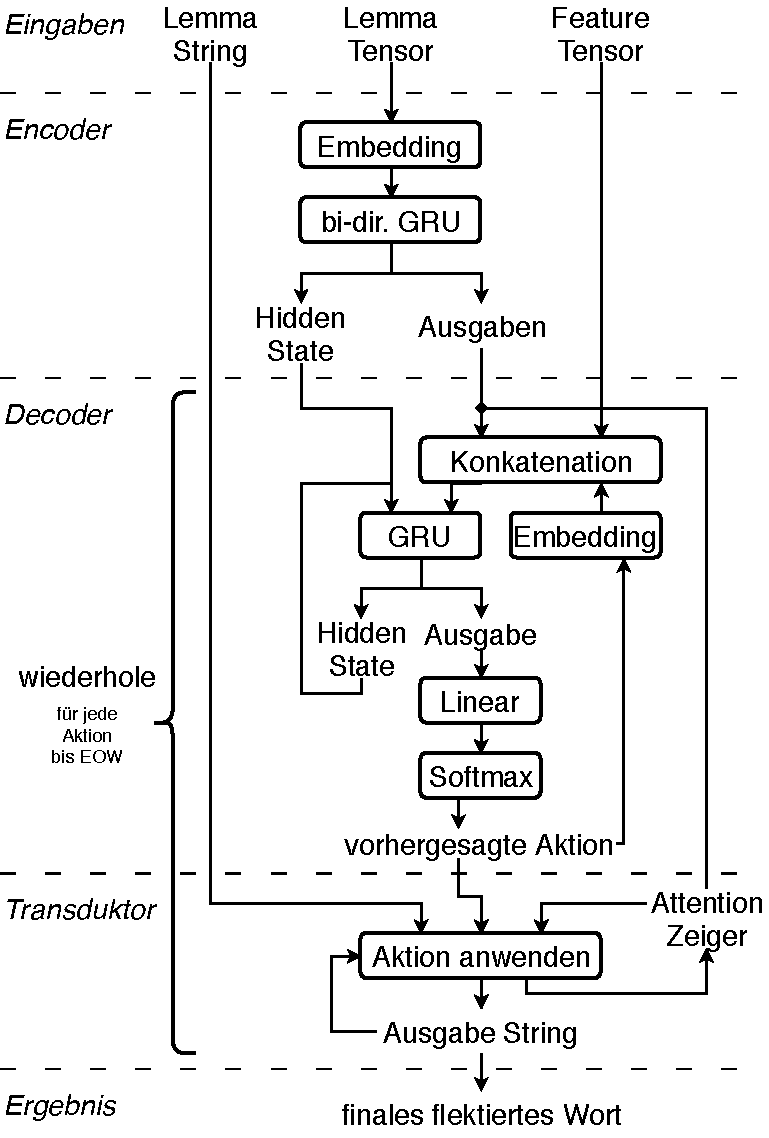
\includegraphics[width=\linewidth]{architecture_de}
\caption{System-Architektur}
\label{fig:arch}
\end{figure}
Die eingesetzte Architektur unseres neuronalen Netzwerkes ist für jede der 103 Sprachen und über die 3 Trainingsdatenmengen hinweg identisch.
Die Architektur des Systems ist in \autoref{fig:arch} dargestellt. Das neuronale Netzwerk agiert dabei als Orakel für den String-Transduktor aus \autoref{sec:transducer}.
Eingaben des gesamten Systems sind das Lemma eines Wortes sowie die Features der gewünschten Flexionsform.
In Abhängigkeit von Lemma, Features, aktueller Position des Zeigers und vorheriger Ausgabe gibt das Netzwerk je eine Aktion (\action{COPY}, \action{PATCH} $p$, \action{MOVE}, \action{EMIT} $s$ oder \action{EOW}) aus, die der String-Transduktor anwendet.
Das Vorhersagen und Anwenden einer Aktion findet für jedes Eingabewort solange statt, bis \action{EOW} durch das neuronale Netzwerk ausgegeben wird. Abschließend finalisiert der String-Transduktor die Flexion des Wortes und gibt sie aus.

In dem neuronalen Netzwerk verwenden wir eine Encoder-Decoder-Struktur \citep{encdec:ChoMGBSB14, seq2seq:SutskeverVL14}, wie sie üblich ist um eine Sequenz in eine andere Sequenz zu überführen; maschinelle Übersetzung stellt einen der wohl geläufigsten Anwendungsfälle dieser Architektur dar.
Der Decoder wendet sich monoton den einzelnen Zeichenrepräsentationen des Lemmas zu, da sich dies in vorherigen Untersuchungen für die Aufgabenstellung der morphologischen Flexion als vorteilhaft erwiesen hat \citep{hardattention:AharoniG16,hardattention:AharoniEtAl}.
Zusätzlich ermöglicht dieses Vorgehen es unserem System, die \action{COPY} und \action{PATCH} Operationen sinnvoll anzuwenden, da zu jeden Zeitpunkt klar ist, welches Eingabezeichen jeweils kopiert bzw. gepatcht werden soll.

Sowohl der Encoder als auch der Decoder bestehen im Kern aus einer einzelnen Gated Recurrent Unit (GRU), die von \citet{encdec:ChoMGBSB14} als einfachere Alternative zu Long Short-Term Memory (LSTM) entwickelt wurden.
Für jedes Zeichen erstellen Embedding-Einheiten numerische Repräsentationen als Eingabe für die beiden GRUs.
Der Encoder verwendet eine bidirektionale GRU, deren Ausgaben aus beiden Richtingen aufsummiert werden, damit auf beide Informationen auf einmal zugegriffen werden kann.
Da der Decoder unidirektional ist, verwenden wir nur den Vorwärtsweg des Encoder-Zustands um den Decoder zu initialisieren.
Im Decoder werden die Zeichen-Embeddings, der betrachtete Kontext und die Features als Tensoren konkateniert und diese Kombination als Eingabe für die GRU genutzt.
Die Ausgabe der GRU im Decoder durchläuft eine lineare Transformation gefolgt von einer logarithmischen Softmax-Operation, um die Netzausgabe auf logarithmische Wahrscheinlichkeiten je Transduktor-Aktion umzusetzen. 

Bias und Gewichte für die GRUs und lineare Transformation sind zufällig anhand einer uniformen Verteilung $\mathcal{U}(-\sqrt{1/s}, \sqrt{1/s})$ initialisiert. Dabei ist $s$ die Größe des internen Zustands einer GRU bzw. die Anzahl der Eingabe-Features. Die Embedding-Gewichte sind ebenso zufällig anhand einer Normalverteilung $\mathcal{N}(0, 1)$ initialisiert.

Für die Verarbeitung eines Wortes, sei es Training oder Vorhersage, werden die nachfolgenden Schritte durchgeführt.
Der Encoder verarbeitet das komplette Eingabe-Lemma als indexbasierten Tensor auf einmal. Dabei generiert dieser Ausgabe-Repräsentationen für jeden Eingabe-Buchstaben sowie eine Repräsentation des internen Zustandes für die gesamte Eingabe-Sequenz.
Durch Verwendung einer externen Schleife produziert der Decoder eine einzelne Transduktor-Aktion pro Schleifendurchlauf.
In jedem Schritt erhält der Decoder als Eingabe seinen vorherigen internen Zustand, die zuletzt ausgegebene Aktion, die Features der Zielform und den zurzeit betrachteten Teil der Encoder-Ausgabe. Auf welchen Teil der Encoder-Ausgabe Zugriff gewährt wird, bestimmt dabei der Index-Zeiger im Transduktor.
Immer, wenn der Decoder eine \action{MOVE} Aktion ausgibt, wird der Index-Zeiger um $1$ erhöht, sodass der Decoder im folgenden Schleifendurchlauf auf die Encoder-Ausgabe für das nächste Lemma-Zeichen zugreift.
Falls Aktionen den Index-Zeiger über die Länge des Lemmas hinaus schieben würden, werden diese stattdessen ignoriert.

\subsection{Beam Search}
% Fynn

% dreht die Seite nicht, sondern nur die Grafik (leichter Druck, schlecht am Bildschirm)
%\begin{sidewaysfigure}[htbp]
%\centering
%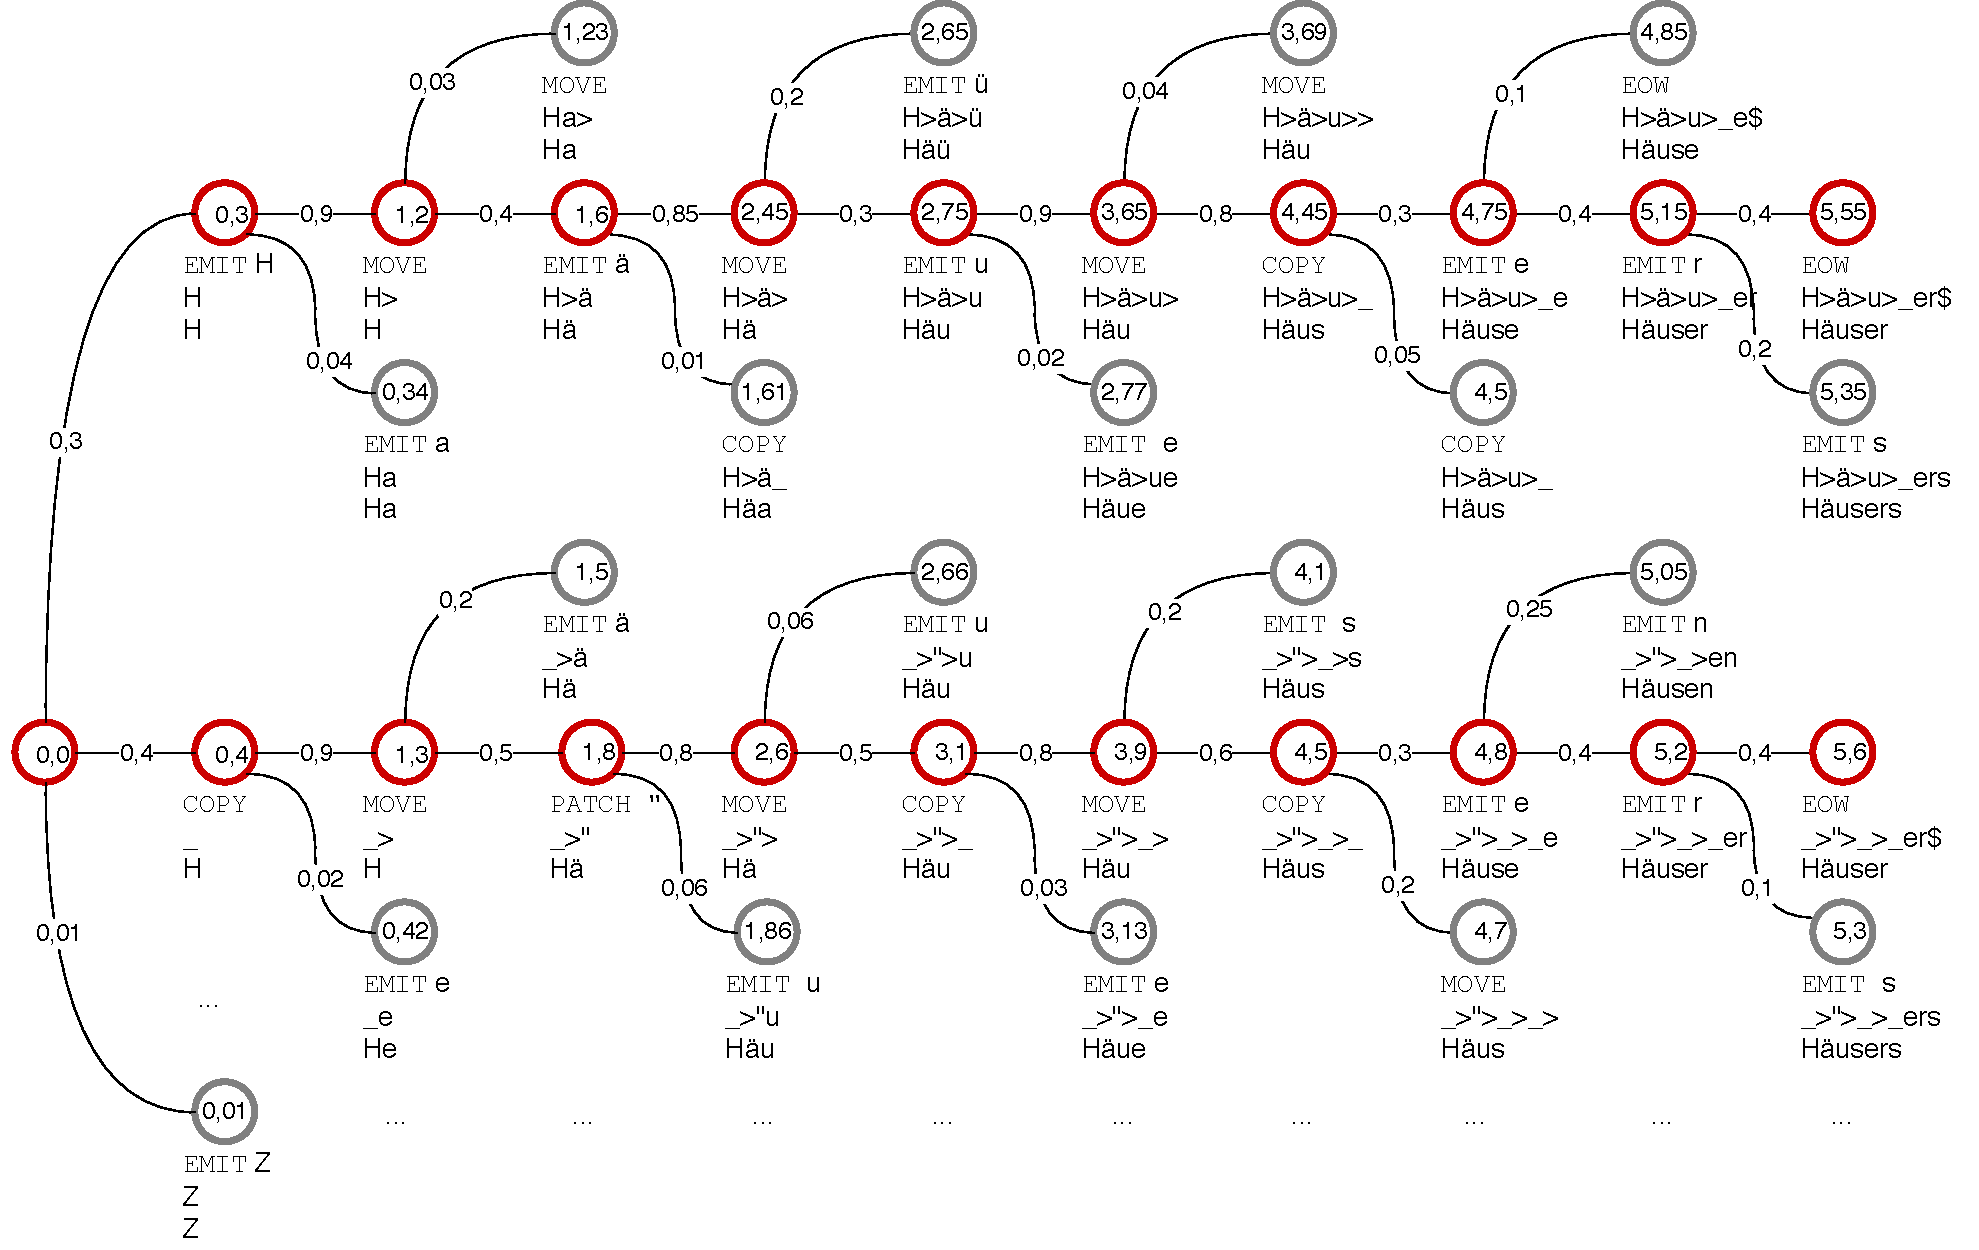
\includegraphics[width=\linewidth, height=\textheight,keepaspectratio]{beam_search}
%    \caption{Beispielhafter Beamsearch Decoding-Prozess}
%    \label{fig:beam}
%\end{sidewaysfigure}

% dreht eine ganze Seite
%\afterpage{
%\begin{landscape}
%  \begin{figure}[htbp]
%  \centering
%    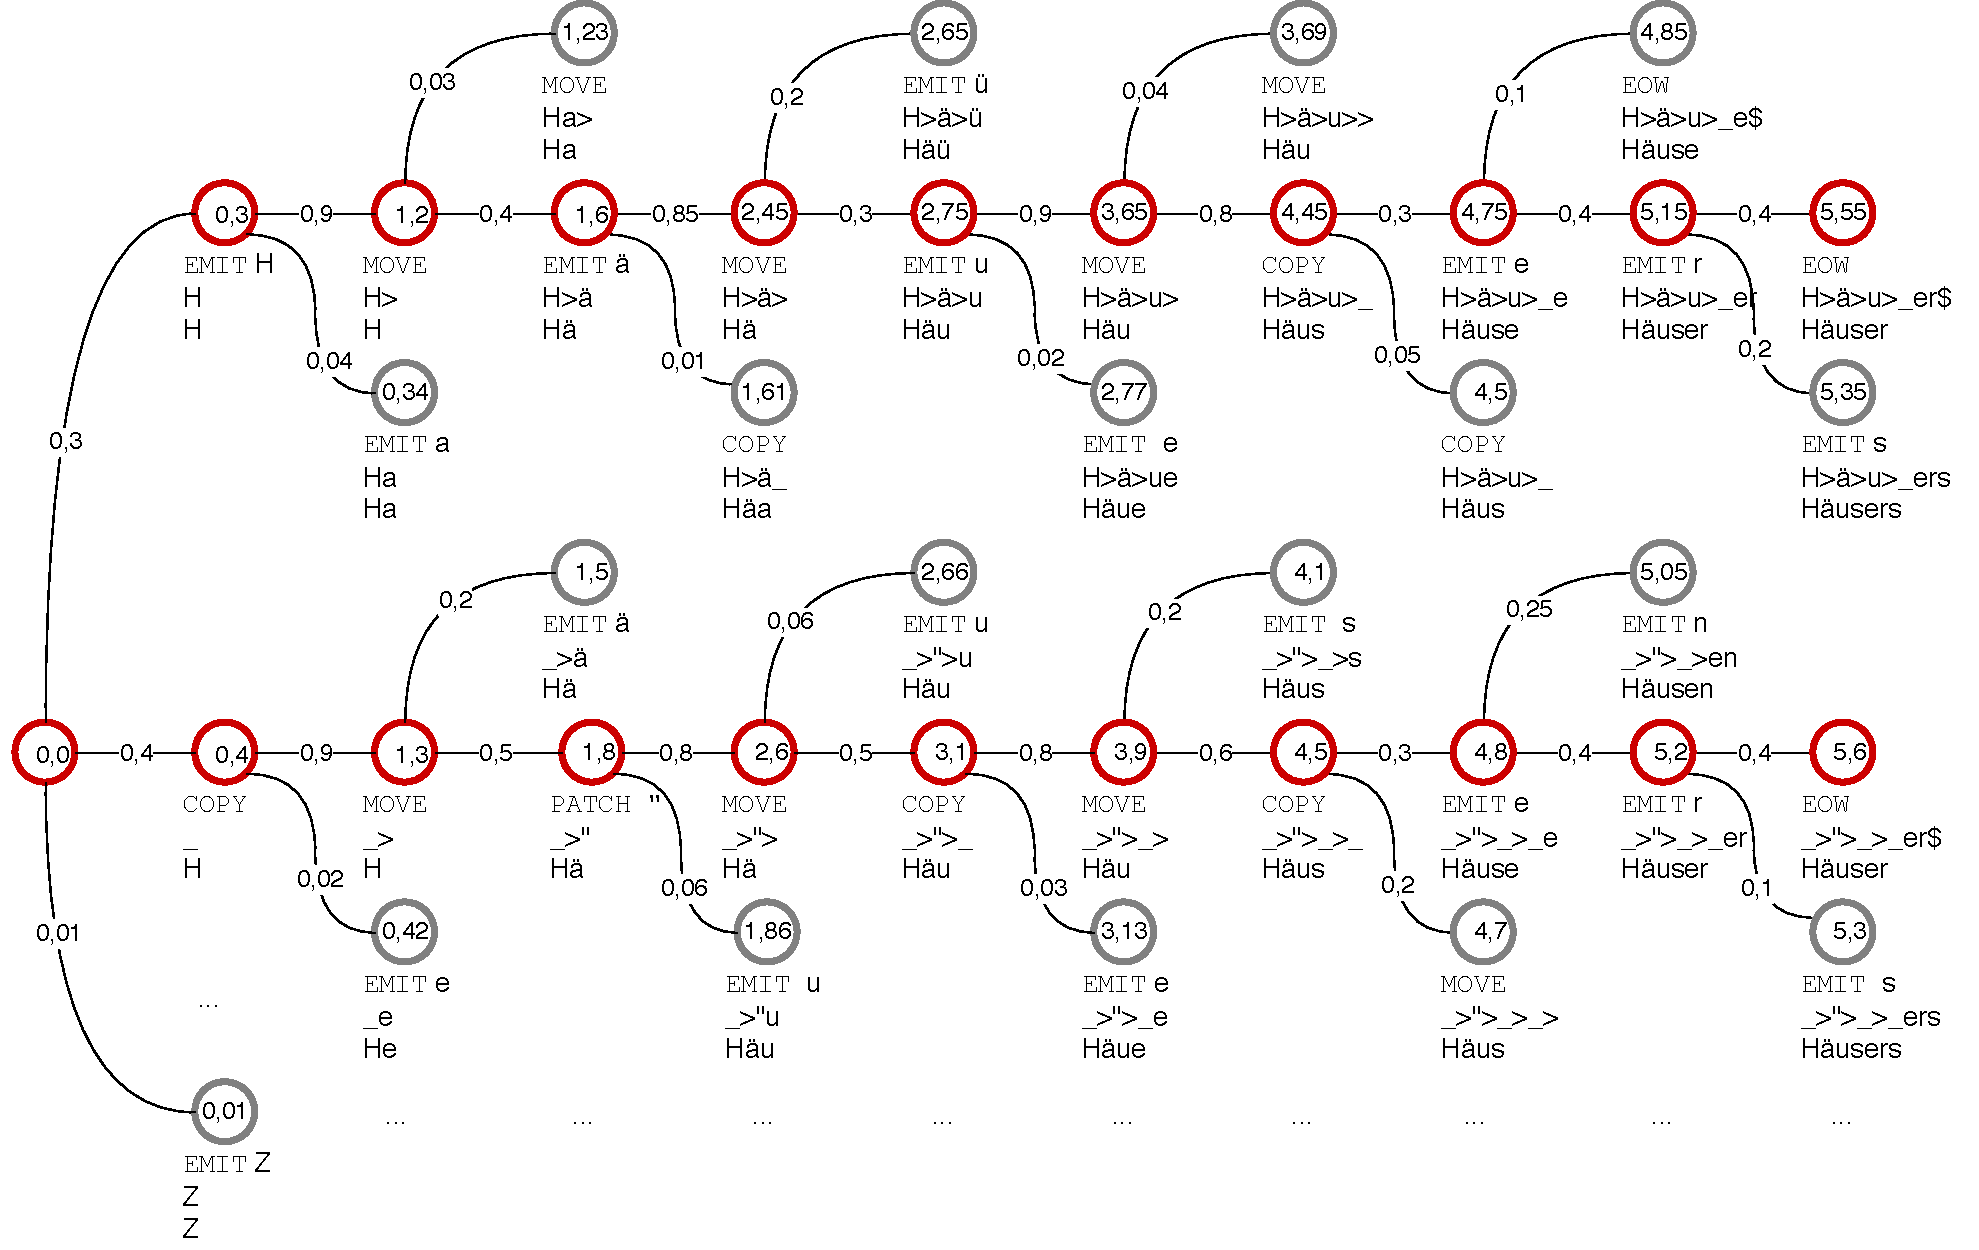
\includegraphics[width=\linewidth, height=\textheight,keepaspectratio]{beam_search}
%    \caption{Beispielhafter Beamsearch Decoding-Prozess von Haus zu Häuser mit Beam-Anzahl 2}
%    \label{fig:beam}
%  \end{figure}
%\end{landscape}
%}
\begin{sidewaysfigure*}[htbp]
  \centering
  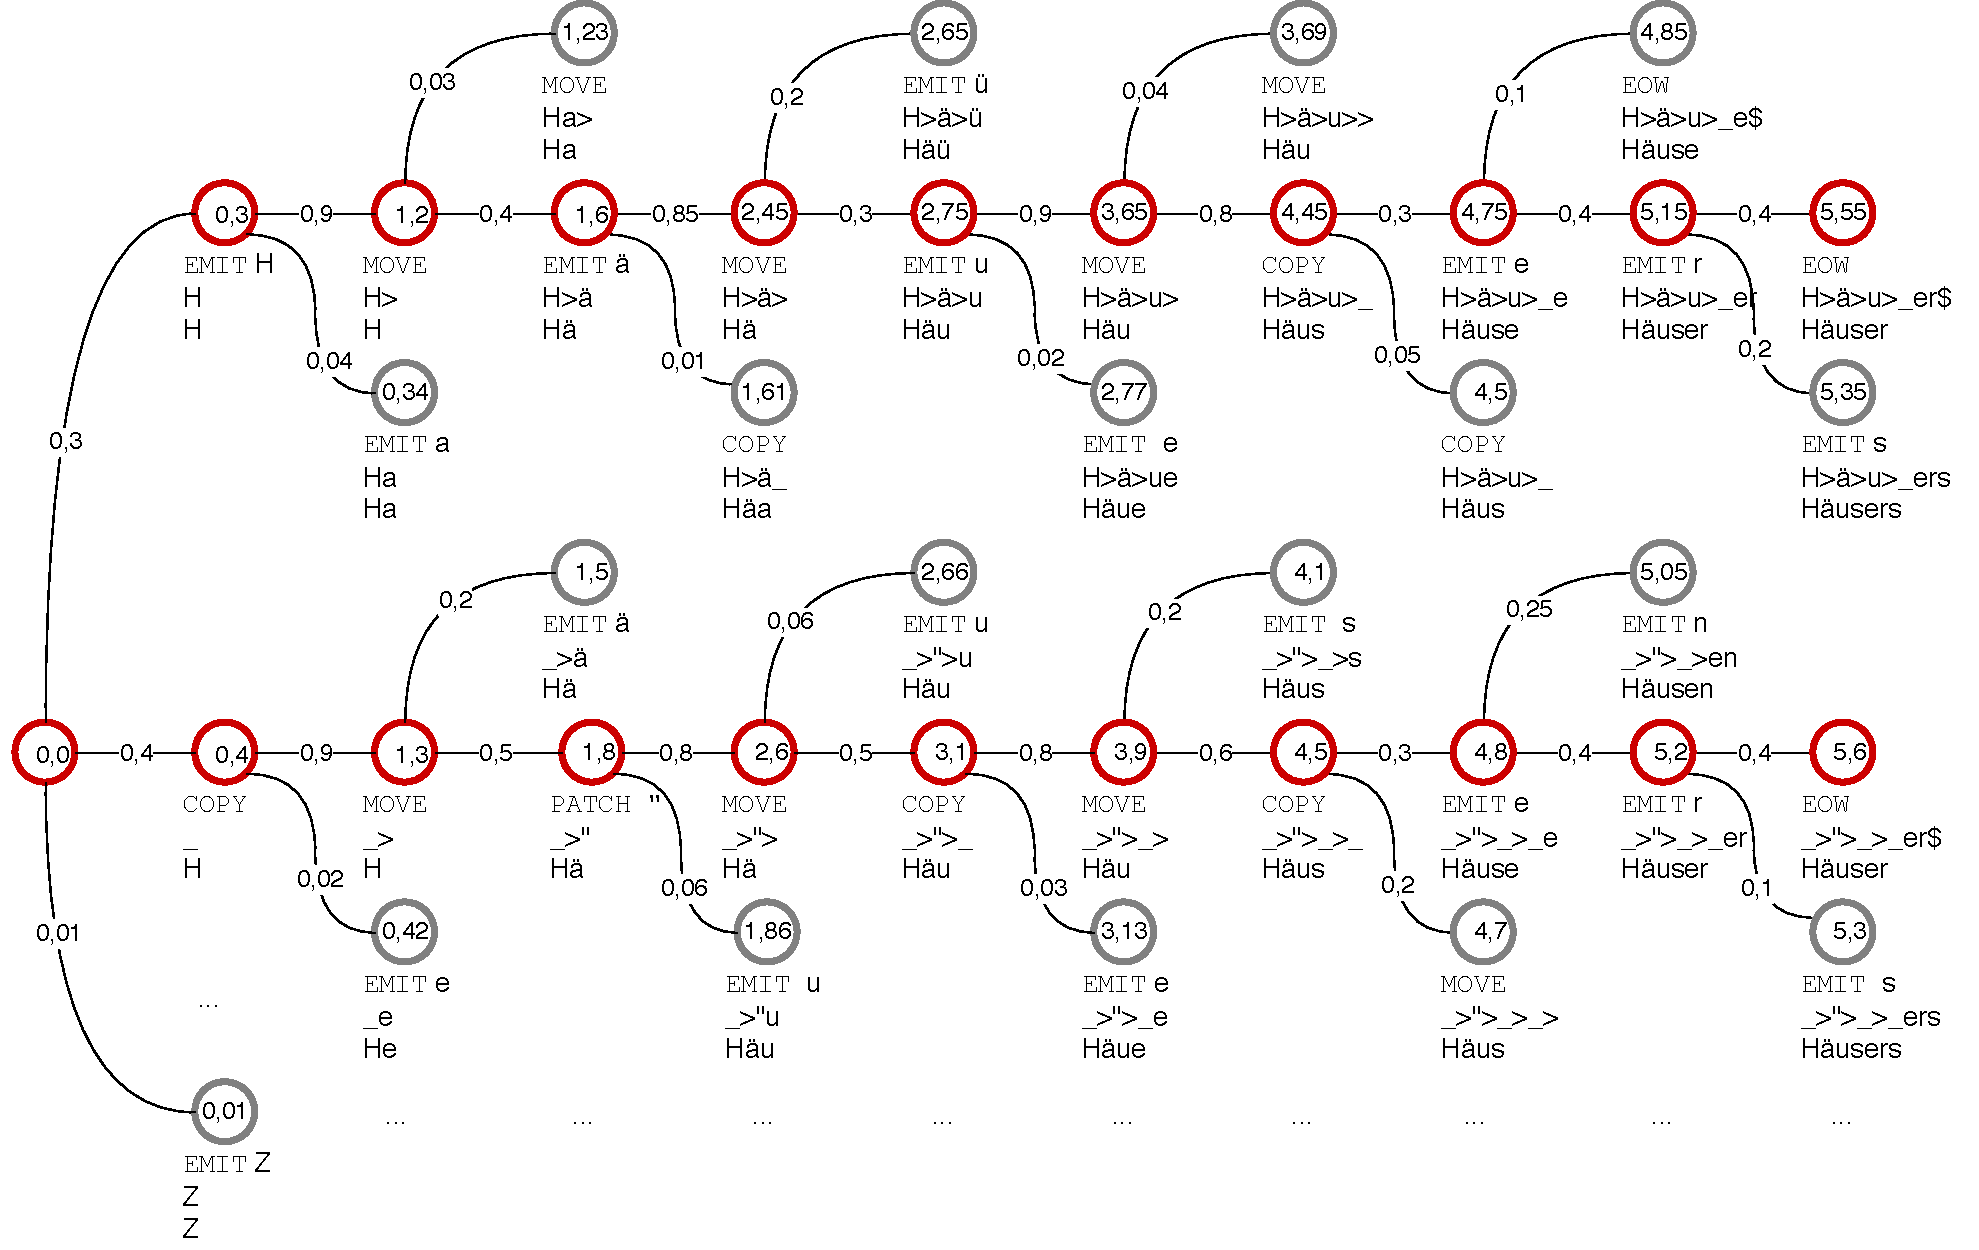
\includegraphics[width=\textwidth-\baselineskip-\abovecaptionskip-\belowcaptionskip,keepaspectratio]{beam_search}
  \caption{Beispielhafter Beam Search Decoding-Prozess von \textit{Haus} zu \textit{Häuser} mit Beam-Anzahl 2}
  \label{fig:beam}
\end{sidewaysfigure*}

Um die Vorhersagegenauigkeit unseres Systems zu verbessern haben wir Beam Search in den Decoding-Prozess eingebaut.
Dies resultiert in mehreren Pfaden, von denen der Pfad mit der größten Wahrscheinlichkeit ausgewählt wird, um das final flektierte Ausgabewort zu erstellen.
Die dazu benötigten Informationen werden in einem zusätzlichen Transduktor-Zustands-Objekt vorgehalten.
Letzteres umfasst den internen Zustand des Decoders, die vorhergesagte Aktion mitsamt ihrer logarithmischen Wahrscheinlichkeit sowie den resultierenden Ausgabe-String für jeden Einzelschritt und Pfad im Decoding-Beam.

\autoref{fig:beam} zeigt einige Pfade eines beispielhaften Decoding-Prozesses, in dem das Lemma \texttt{Haus} in die Pluralform \texttt{Häuser} überführt werden soll.
Die Kreise stellen einzelne Zustände für jeden Zeitschritt dar.
Die Zahl im Inneren ist die logarithmische Wahrscheinlichkeit des Zustandes, die entlang der Pfade von links nach rechts aufsummiert wird.
Das Beispiel zeigt einen Decoding-Prozess mit einer Beam-Anzahl von $2$, und die aktiven Pfade sind durch rote Kreise markiert.
Die Zahl an einer Kante zwischen zwei Zuständen gibt die logarithmische Wahrscheinlichkeit für die Aktion unterhalb eines jeden Kreises für den jeweils nachfolgenden Zustand an.
In den Zeilen darunter ist die aktuelle Aktionssequenz sowie das Ergebnis der Anwendung auf das Lemma dargestellt.
Für die Aktionssequenz gelten folgende Abkürzungen: \texttt{\_} entspricht \action{COPY}, \texttt{>} ist \action{MOVE}, \texttt{\"} ist die \action{PATCH} Aktion mit Umlaut und Buchstaben gelten als \action{EMIT} des jeweiligen Zeichens.

Der Decoding-Prozess in \autoref{fig:beam} startet in einem initialen Startzustand mit log. Wahrscheinlichkeit $0$.
Das neuronale Netzwerk gibt für jede mögliche Aktion die log. Wahrscheinlichkeit an, wobei \action{COPY} in diesem Fall die höchste Wahrscheinlichkeit hat.
Da zwei aktive Pfade verfolgt werden, ist auch der Zustand der zweitwahrscheinlichsten Aktion \action{EMIT H} aktiv.
In jedem Zeitschritt wird nun für jeden aktiven, aktuellen Zustand die Menge der möglichen Folgezustände mit ihren jeweiligen Wahrscheinlichkeiten berechnet.
Aus der Gesamtmenge der neuen Zustände in diesem Zeitschritt werden dann die zwei (maximale Beam-Anzahl) mit der höchsten Wahrscheinlichkeit ausgewählt, die Übrigen verworfen.
Dadurch bilden sich Pfade mit diversen abgebrochenen Abzweigungen heraus, die die höchste aufsummierte log. Wahrscheinlichkeit innehaben.
Dieses Vorgehen wird solange fortgesetzt bis zwei Pfade zum Ende (Aktion \action{EOW}) gelangen.
Aus diesen wird nun der beste Pfad (mit höchster log. Wahrscheinlichkeit) ausgewählt, um die finale Ausgabe der Flexion zu erstellen.
In diesem Fall ist dies der untere rote Pfad, welcher \texttt{Haus} nach \texttt{Häuser} mittels der Aktionskette \action{COPY} \action{MOVE} \action{PATCH "} \action{MOVE} \action{COPY} \action{MOVE} \action{COPY} \action{EMIT e} \action{EMIT r} überführt.

Der große Vorteil des Beam-Decodings liegt darin, bessere Lösungen als das gierige Dekodieren (\textit{greedy decoding}) zu finden, indem mehrere Pfade gleichzeitig weiterverfolgt werden.
Wenn der Pfad mit der initial höchsten Wahrscheinlichkeit sich später als absolut unbrauchbar heraus stellt, treten im Beam-Decoding andere Pfade an seine Stelle und führen so zu einem meist besseren Ergebnis.
Die Auswirkungen von Beam-Decoding auf die Ergebnisse unseres Systems werden in \autoref{sec:beam-results} vorgestellt.

Für die Verbesserung der Vorhersage mittels Beam-Decoding wird allerdings auch eine erhöhte Rechenleistung erfordert: Der Aufwand des Decoders steigt in etwa linear mit der Beam-Anzahl an. 
Diese Kosten sind jedoch nur in der finalen Evaluation zu zahlen, da während des Trainings kein Beam-Decoding stattfinden muss.
Es kann jedoch auch dazu verwendet werden, das Training des Netzwerkes zu verbessern wie in \autoref{sec:training} erläutert wird.

\subsection{Training}
\label{sec:training}
% Fynn

Da das neuronale Netzwerk eine Sequenz von Transduktor-Aktionen ausgibt, handelt es sich bei den Trainingszielen nicht um flektierte Wörter, sondern ebenfalls um Aktionssequenzen, die die eigentlichen Flexionen produzieren, wenn sie auf das Lemma angewandt werden.
Diese Aktionssequenzen werden zuvor von unserem System erzeugt, indem im Gleichschritt über das alignierte Lemma und das flektierte Wort iteriert wird.
Für jede Zeichenkombination werden die zugehörigen Aktionen der neuen Ausgabesequenz hinzugefügt.
Der Algorithmus ist im Detail in \autoref{sec:orakel-alg} beschrieben.

Trainingsschritte werden mittels Backpropagation durch den Adam Optimierer \citep{adam:KingmaB14} durchgeführt.
Dieser ist mit den folgenden Paramtern konfiguriert: \textit{Learning rate} $\alpha=0.005$, \textit{Momentum Decays} $\beta_1=0.9$, $\beta_2=0.999$, \textit{Numerical Stabilizer} $\epsilon=10^{-8}$ und \textit{Weight Decay} (L2 Regularisierung) von $0.001$.

Das implementierte Beam-Decoding erlaubt theoretisch eine globale Normalisierung des neuronalen Netzwerks nach \citet{globalnorm:AndorAWSPGPC16}.
Leider konvergiert das Training des Modells mit globaler Normalisierung und Beam Search in unseren Versuchen nicht.
\citet{globalnorm:AndorAWSPGPC16} haben vortrainierte Gewichte mittels lokaler Normalisierung verwendet, um dieses Problem zu umgehen.
Da wir allerdings keine robuste Möglichkeit zum Wechseln von lokaler zu globaler Normalisierung für alle 103 Sprachen finden konnten, setzen wir ausschließlich lokale Normalisierung im Training ein.
Sobald der korrekte Pfad während des Dekodierens aus dem Beam fällt, wird ein Trainingsupdate mit unserer spezifischen \textit{Loss}-Funktion auf Grundlage der logarithmischen Wahrscheinlichkeiten der Schritte im korrekten Pfad durchgeführt.

Die \textit{Loss}-Funktion in \autoref{eq:loss} basiert auf der lokal normalisierten Pfadwahrscheinlichkeit, die als Gleichung (4) in \citet{globalnorm:AndorAWSPGPC16} dargestellt ist.
Sie berechnet die negative Summe über die logarithmischen Wahrscheinlichkeiten $l$ der korrekten Aktionen für jeden Schritt des Pfades.
Das Dividieren durch den natürlichen Logarithmus der Sequenzlänge $s$ führt zu gleichmäßigeren \textit{Loss}-Größenordnungen, was dem Trainingsprozess hilft besser zu konvergieren.
Wir vermuten, dass dies der Fall ist, da wir die Fehler über alle Schritte aufsummieren, wozu auch diejenigen korrekten Vorhersagen zählen bei denen das System nicht zu 100 \% sicher ist.
Das berechnete Ergebnis $L$ der Funktion wird anschließend verwendet, um die Trainingsupdates mittels \textit{Backpropagation} zurück durch das gesamte neuronale Netzwerk zu führen.

\begin{equation}
\label{eq:loss}
L = - \frac{\sum_i^s l_i}{\ln{(1+s)}}
\end{equation}

Durch den Verzicht auf globale Normalisierung und die Verwendung von lokaler Normalisierung konnten wir das Konvergieren des Lernprozesses wiederherstellen. Allerdings konnten wir dadurch keine signifikanten Vorteile in der Verwendung mehrerer Beams während des Trainings finden.
Eine mögliche Erklärung weshalb unser Netzwerkmodell im Training nicht von Beam-Decoding profitiert ist, dass das Modell viele Trainingsupdates erfordert.
Während durch das Bestrafen korrekter Schritte des Decoding-Prozesses viele Trainingsupdates entstehen, könnten selbige bei Beam-Decoding zu selten stattfinden, da mit höherer Wahrscheinlichkeit mindestens ein korrekter Pfad im Beam vorhanden ist.

Zur Abgabe der Daten für den Shared Task haben wir auf Beam-Decoding verzichtet, indem wir als Anzahl der Pfade $1$ verwendet haben.
Die entwickelte Architektur ist allerdings bereit sowohl Beam-Decoding als auch globale Normalisierung zu verwenden.
Auf dieser Grundlage haben wir auch noch weitere Untersuchungen vorgenommen, die später vorgestellt werden.
So ist beispielsweise auch das Trainieren mit einem einzigen Pfad und gleichzeitiges Evaluieren mit mehreren Pfaden möglich. Dadurch kann die Vorhersage verbessert werden, ohne die Trainingslaufzeit zu erhöhen.
Aufgrund der relativ komplexen Implementierung des Beam-Decoding haben wir bis zur Abgabe des Shared Tasks kein Mini-Batching implementiert. Nachträglich ist jedoch auch Mini-Batching eingebaut worden, um das Training hinsichtlich Konvergenz und Rechner-Ressourcenauslastung zu optimieren.

\section{Feinabstimmung und Evaluation}
\label{sec:tuning_evaluation}
% Fynn

\begin{table*}[htb]
    \centering
    \begin{tabularx}{\textwidth}{lcX}
    \toprule
    Parameter & Werte & Beschreibung\\
    \midrule
        GRU Größe & 32, 64, 128 & Tensor Größe des internen Zustands von Encoder \& Decoder\\
        Embedding Größe & 8, 16 & Tensor Größe der Zeichen-Embeddings\\
        Patches & ja, nein & Verwendung der Patches aktiv?\\
        Enhancer & 0\times, 1\times, 5\times & Faktor der Erzeugung zusätzlicher Trainingsdaten\\
    \bottomrule
    \end{tabularx}
    \caption{Hyperparameter}
    \label{tab:params}
\end{table*}

Um die Ergebnisse unseres Systems zu verbessern, haben wir eine ausgedehnte Hyperparameter-Suche vorgenommen.
Der zuvor geschilderte Aufbau des Systems ist dabei für alle Sprachen identisch.
Je Sprache und Größe des Trainingsdatensatzes haben wir eine unabhängige Hyperparameter-Suche auf einer zufälligen Auswahl aus dem Such-Raster der Parameter durchgeführt.
\autoref{tab:params} listet die Hyperparameter mit möglichen Werten auf.

Während der Entwicklungsphase des Systems ist uns aufgefallen, dass die zufällige Initialisierung der Netzwerkgewichte großen Einfluss auf die Ergebnisse hat. Es handelt sich dabei um ein typisches Problem, welches insbesondere dann auftritt, wenn nur wenige Trainingsdaten zur Verfügung stehen.
Aus diesem Grund wird in unserer Hyperparamter-Suche jede Parameterkombination mit fünf verschiedenen Zufalls-Seeds durchlaufen, wodurch sowohl die Netzwerkgewichte andere Startwerte annehmen als auch die Reihenfolge der einzelnen Trainingsdatenpunkte variiert.

Die Hyperparameter-Suche erstreckt sich insgesamt über 103 Sprachen, 3 Trainingsdatensätze, 3 GRU-Größen, 2 Embedding-Größen, 2 Patch-Zustände, 3 Enhancer-Stufen und 5 Zufalls-Seeds, was in $103 \times 3 \times 3 \times 2 \times 2 \times 3 \times 5 = 55.620$ Parameterkombinationen resultiert.
Jeder einzelne Durchlauf erfordert ein vollständiges Training des neuronalen Netzwerkes sowie die Erzeugung der Ausgabedaten.
Dies dauert in etwa ein bis drei Minuten für den kleinsten, zehn bis 20 Minuten für den mittleren und ein bis zwei Stunden für den größten Trainingsdatensatz.

Da eine erschöpfende Suche von $55.620$ Parameterkombinationen zu viel Rechenzeit in Anspruch nähme, haben wir Möglichkeiten erkundet um den Suchaufwand zu reduzieren. Für den mittleren Trainingsdatensatz werden nur GRU- und Embedding-Größen getestet, die größer oder gleich dem besten Ergebnis auf dem kleinen Trainingsdatensatz sind.
Analog dazu ist der große Datensatz ebenfalls in diesen beiden Parametern durch die besten Ergebnisse des mittleren Datensatzes beschränkt.
Dies ist naheliegend, da mit steigender Anzahl von Gewichten im neuronalen Netzwerk mehr Trainingsdaten benötigt werden, damit kein \textit{Overfitting} eintritt.
Zusätzlich verwenden wir den Enhancer ausschließlich auf dem kleinen Trainingsdatensatz, da bereits das mittlere Set genügend Trainingsbeispiele enthält.
Aus diesen reduzierten Parameterkombinationen wird je Sprache und Größe der Trainingsdaten eine zufällige Auswahl gezogen, um eine feste obere Grenze an Trainingsdurchläufen zu garantieren.
Für die Abgabe der Ergebnisse für den Shared Task hat unsere Hyperparameter-Suche $9.278$ Trainingsläufe durchgeführt, was einer Reduktion auf beinahe ein Sechstel der ursprünglichen Menge entspricht.

Während einer frühen Evaluation der Ergebnisse konnten wir feststellen, dass unser System in der Vorhersage manchmal das Wort nicht mit \action{EOW} beendet und stattdessen endlos den letzten Buchstaben des Lemmas mit \action{COPY} kopieren möchte oder gar ein beliebiges Zeichen mit \action{EMIT} andauernd wiederholt.
Daher enthält der String-Transduktor Maßnahmen um diese Probleme zu entschärfen.
Wenn der Zeiger bereits über das Eingabewort hinaus bewegt wurde, greifen folgende Regelungen:
Die Aktionen \action{COPY} und \action{PATCH} werden nicht mehr angewandt. Die \action{EMIT} Aktion kann das zuvor geschriebene Zeichen nicht erneut ausgeben. 
Dadurch können jedoch die flektierten Formen in einigen Ausnahmefällen einzelne Zeichen am Ende vermissen. 

Für die finale Evaluation der Testdatensätze haben wir die beste Parameterkombination (inklusive Zufalls-Seed) für jedes Paar aus Sprache und Größe auf Basis der jeweiligen Levenshtein-Distanz der Ergebnisse auf dem bereitgestellten Entwicklungsdatensatz verwendet.

\section{Ergebnisse und Diskussion}
\label{sec:results}

% \todo[inline]{Ist doch eigentlich ungeil, direkt unter eine sec Überschrift eine subsec zu packen?? Mir fällt leider kein knackiger Einleitungstext ein -- Gregor}
In diesem Abschnitt vergleichen wir die Ergebnisse unseres Systems mit anderen Einreichungen, evaluieren den Effekt von Patches, Enhancer sowie Beam-Decoding und analysieren die Ursachen der Schwachstellen unseres Systems.

\subsection{Eingereichte Ergebnisse}
\label{sec:eingereichte_ergebnisse}

\begin{table*}[tbh]
% Fynn
\newcommand{\incompl}[1]{\color{gray}#1}
\newcommand{\wir}[1]{\textbf{#1}}
\newcommand{\bl}[1]{\textit{#1}}
\begin{tabular}{lc|lc|lc}
\toprule
\multicolumn{2}{c}{high}                  & \multicolumn{2}{c}{medium}                & \multicolumn{2}{c}{low}                        \\
\midrule
uzh             & 96.00 / 0.08            & uzh             & 86.64 / 0.26            & uzh                   & 57.21 / 1.02           \\
bme             & 94.66 / 0.11            & iitbhu-iiith    & 84.19 / 0.32            & iitbhu-iiith          & 52.60 / 1.10           \\
iitbhu-iiith    & 94.43 / 0.11            & \wir{hamburg}   & \wir{74.03 / 0.54}      & ua                    & 53.22 / 1.35           \\
iit-varanasi    & 91.73 / 0.16            & msu             & 76.40 / 0.55            & \wir{hamburg}         & \wir{40.28 / 1.45}     \\
waseda          & 91.12 / 0.19            & iit-varanasi    & 70.17 / 0.66            & waseda-01             & 44.09 / 1.68           \\
msu             & 91.87 / 0.23            & waseda          & 77.38 / 0.67            & msu                   & 41.61 / 1.86           \\
axsemantics     & 84.19 / 0.40            & bme             & 67.43 / 0.75            & \bl{baseline}         & \bl{38.89} / \bl{1.88} \\
\wir{hamburg}   & \wir{77.53 / 0.44}      & \bl{baseline}   & \bl{63.53} / \bl{0.90}  & iit-varanasi          & 23.33 / 2.40           \\
\bl{baseline}   & \bl{77.42} / \bl{0.51}  & axsemantics     & 60.00 / 1.03            & tuebing.-oslo        & \ 4.43 / 5.06             \\
tuebing.-oslo  & 63.05 / 1.15             & tuebing.-oslo  & 30.98 / 2.25             & bme                   & \ 3.74 / 6.72            \\
\incompl{racai} & \incompl{79.93 / 0.43}  & \incompl{kucst} & \incompl{32.28 / 2.23}  & \incompl{axsemantics} & \incompl{14.89 / 3.89} \\
\incompl{kucst} & \incompl{54.37 / 1.57}  & \incompl{ua}    & \incompl{\ \ --- / ---} & \incompl{kucst}       & \incompl{\ 2.79 / 5.28}\\
\incompl{ua}    & \incompl{\ \ --- / ---} & \incompl{racai} & \incompl{\ \ --- / ---} & \incompl{racai}       & \incompl{\ \ --- / ---}\\

\bottomrule
\end{tabular}
\caption{Durchschnittliche Ergebnisse über alle 103 Sprachen als Accuracy (Prozentpunkte) / mittlere Levensthein-Distanz (von der korrekten Form in Zeichen) aller Teilnehmer am Shared Task 2018.
Sofern Teilnehmer mehrere Systeme eingereicht haben, wird nur das je Trainingsdatenmenge beste System aufgeführt.
Die Zeilen sind je Trainingsdatenmenge nach Levensthein-Distanz aufsteigend sortiert.
Ausgegraute Einträge repräsentieren unvollständige Einreichungen, die sich nicht sinnvoll vergleichen lassen und daher immer am Ende gelistet werden.
Ergebnisse sind aus Tabelle 8 in \citet{sigmorphon:st2018} entnommen.}
\label{fig:results_all}
\end{table*}

%\begin{table*}[tbh]
%%\small
%\centering
%\begin{tabular}{lr|lr|lr}
%\toprule
%\textbf{high}             & & \textbf{medium}                 &  & \textbf{low}                  &  \\
%\midrule
%Teilnehmer                 & Accuracy                    & Teilnehmer                & Accuracy                      & Teilnehmer                & Accuracy
%\\
%\rule{0pt}{3ex}uzh-01                     & 96                     & uzh-01                     & 86.64                   & uzh-02                     & 57.21                  \\
%uzh-02                     & 95.97                  & uzh-02                     & 86.38                   & uzh-01                     & 57.18                  \\
%bme-02                     & 94.66                  & iitbhu-iiith-02            & 84.19                   & ua-08                      & 53.22                  \\
%iitbhu-iiith-02            & 94.43                  & iitbhu-iiith-01            & 82.9                    & iitbhu-iiith-02            & 52.6                   \\
%iitbhu-iiith-01            & 94.43                  & waseda-01                  & 77.38                   & ua-05                      & 50.53                  \\
%bme-03                     & 93.97                  & msu-04                     & 76.4                    & iitbhu-iiith-01            & 49.79                  \\
%bme-01                     & 93.88                  & msu-03                     & 75.74                   & ua-06                      & 49.73                  \\
%msu-04                     & 91.87                  & \textbf{hamburg-01}        & \textbf{74.03}          & ua-03                      & 44.82                  \\
%iit-varanasi-01            & 91.73                  & iit-varanasi-01            & 70.17                   & waseda-01                  & 44.09                  \\
%waseda-01                  & 91.12                  & msu-02                     & 69.45                   & msu-02                     & 41.61                  \\
%msu-03                     & 90.52                  & bme-01                     & 67.43                   & \textbf{hamburg-01}        & \textbf{40.28}         \\
%axsemantics-01             & 84.19                  & bme-03                     & 67.36                   & ua-02                      & 39.19                  \\
%msu-02                     & 82.68                  & bme-02                     & 67.26                   & ua-01                      & 38.22                  \\
%\textbf{hamburg-01}        & \textbf{77.53}         & \textit{\textbf{baseline}} & \textit{\textbf{61.78}} & \textit{\textbf{baseline}} & \textit{\textbf{38.2}} \\
%\textit{\textbf{baseline}} & \textit{\textbf{75.3}} & axsemantics-02             & 60                      & ua-07                      & 37.99                  \\
%axsemantics-02             & 74.77                  & msu-01                     & 54.44                   & msu-04                     & 31.4                   \\
%msu-01                     & 74.33                  & tuebingen-oslo-03          & 30.98                   & msu-03                     & 25.86                  \\
%racai-01                   & 72.49                  & tuebingen-oslo-02          & 29.72                   & iit-varanasi-01            & 23.33                  \\
%tuebingen-oslo-03          & 63.05                  & kucst-01                   & 29.12                   & ua-04                      & 21.25                  \\
%tuebingen-oslo-02          & 56.6                   & tuebingen-oslo-01          & 20.97                   & axsemantics-02             & 14.74                  \\
%tuebingen-oslo-01          & 49.52                  & axsemantics-01             & 9.1                     & tuebingen-oslo-02          & 4.43                   \\
%kucst-01                   & 48.68                  & ua-08                      & 0                       & bme-01                     & 3.74                   \\
%ua-08                      & 0                      & ua-07                      & 0                       & bme-03                     & 3.63                   \\
%ua-07                      & 0                      & ua-06                      & 0                       & kucst-01                   & 2.52                   \\
%ua-06                      & 0                      & ua-05                      & 0                       & bme-02                     & 2.43                   \\
%ua-05                      & 0                      & ua-04                      & 0                       & tuebingen-oslo-03          & 1.39                   \\
%ua-04                      & 0                      & ua-03                      & 0                       & axsemantics-01             & 0.7                    \\
%ua-03                      & 0                      & ua-02                      & 0                       & tuebingen-oslo-01          & 0                      \\
%ua-02                      & 0                      & ua-01                      & 0                       & racai-01                   & 0                      \\
%ua-01                      & 0                      & racai-01                   & 0                       & msu-01                     & 0         
%\\
%\bottomrule
%\multicolumn{6}{l}{$0$: keine Einreichung des Teilnehmers}
%\end{tabular}
%
%\caption{Ergebnisse (Accuracy) aller Teilnehmer am Shared Task für alle Mengen.
%\todo[inline]{Wir sollten auch die Levensthein Ergebnisse zeigen, insb. für Schwachstellen hilfreich}}
%
%%Abrufbar unter: \url{https://docs.google.com/spreadsheets/d/1HqOGRyltYvji7pi-jq3swEfoWs15k5QU-lA3ua8dpmo/}
%\label{fig:results_all}
%\end{table*}%



\begin{table}
\centering
\begin{tabular}{lrrr}
\toprule
                 & high   & medium & low    \\
                 \midrule
Baseline         & 77.42 & 63.53 & 38.39 \\
Ø Teilnehmer     & 87.17 & 69.69 & 35.61 \\
Wir              & 77.53 & 74.03 & 40.28 \\
\bottomrule
\end{tabular}
\caption{Accuracy (in Prozentpunkten) unserer Ergebnisse im Vergleich zur Baseline sowie dem Durchschnitt der besten, vollständigen Einreichungen je Team.}
\label{fig:acc_comparison}
\end{table}

\begin{table}
\centering
\begin{tabular}{lrrr}
\toprule
         & high & medium & low  \\
         \midrule
Baseline     & 0.51 & 0.90   & 1.88 \\
Ø Teilnehmer & 0.32 & 0.78   & 2.51 \\
Wir          & 0.44 & 0.54   & 1.45\\
\bottomrule
\end{tabular}
\caption{Durchschnittliche Levenshtein-Distanz unserer Ergebnisse im Vergleich zur Baseline sowie dem Durchschnitt der besten (vollständigen) Einreichungen je Team.}
\label{fig:lev_comparison}
\end{table}

% Marcel?, Fynn
In \autoref{fig:results_all} sind die veröffentlichten Ergebnisse der besten Systeme je Team für die drei Trainingsdatenmengen dargestellt. Wir konnten uns auf \textit{medium} und \textit{low} im oberen Drittel platzieren. Auf dem \textit{high} Datensatz liegt unser System jedoch in der unteren Hälfte. Dennoch konnten wir immer unser Ziel erreichen und  die Baseline übertreffen.

Die beste Platzierung (Rang 3 von 10) und die größte Verbesserung im Vergleich zur Baseline ($10.50$ Prozentpunkte) konnten wir mit einer Genauigkeit von $74.03$ Prozentpunkten bzw. Levenshtein-Distanz von $0.54$ auf der mittleren Trainingsdatenmenge erreichen.
Auf \textit{high} und \textit{low} lagen unsere Ergebnisse mit $77.53$ / $0.44$ bzw. $40.28$ / $1.45$ hinsichtlich der Accuracy nur knapp über der Baseline, während wir zumindest auf \textit{low} bei der Levensthein-Distanz einen deutlichen Vorsprung vorweisen können.

In den Tabellen \ref{fig:acc_comparison} und \ref{fig:lev_comparison} sind unsere Ergebnisse nach Accuracy und Levenshtein im Vergleich zur Baseline sowie zum Durchschnitt der anderen Teilnehmer aufgeführt. Wir konnten die durchschnittliche Accuracy der Teilnehmer auf \textit{medium} ($+4.34$) und \textit{low} ($+4.67$) schlagen.
Die Accuracy der Baseline konnten wir auf allen Größenordnungen schlagen. Dies gilt insbesondere auch für die durchschnittliche Levensthein-Distanz.
Besonders auf \textit{medium} ($-0.36$) ist die Verbesserung relativ gesehen mit $40\%$ deutlich, bei \textit{high} ($-0.07$, Verbesserung um $13\%$) und \textit{low} ($-0.43$, Verbesserung um $22\%$) weniger deutlich.
Gegenüber dem Durchschnitt der anderen Teilnehmer fällt unser Vorsprung auf \textit{medium} kleiner, dafür auf \textit{low} größer aus.

\autoref{tab:langs_baseline} zeigt diejenigen Sprachen, die am weitesten \textbf{über} und \textbf{unter} der Baseline lagen. In \autoref{sec:schwachstellen} werden die Schwachstellen des Systems beschrieben, die mit hoher Wahrscheinlichkeit zumindest zum Teil für die schlechten Ergebnisse auf manchen Sprachen verantwortlich sind.

\begin{table}
\centering
\small
\begin{tabular}{llrr}
  \toprule
                           & \textbf{Sprachen}  &\textbf{Wir} & \textbf{BL} \\
\midrule\textbf{Beste}   & Uzbek              & $100.0$      & $96.0$ \\
                           & Mapudungun         & $100.0$      & $82.0$ \\
                           & Classical-Syriac   & $97.0$       & $99.0$ \\
%\midrule
\textbf{Schlechteste}         & Old-Irish          & $6.0$        & $16.0$ \\
                           & Haida              & $16.1$       & $61.0$ \\
                           & Latin              & $21.4$       & $37.6$ \\
%\midrule
\midrule
\textbf{max(Wir - BL)}    & Swahili            & $95.0$         & $0.0$ \\
                           & Murrinhpatha       & $88.0$       & $0.0$ \\
                           & Zulu               & $81.8$       & $0.1$ \\
\textbf{max(BL - Wir)}    & Neapolitan         & $49.0$       & $94.0$ \\
                           & Haida              & $16.0$       & $61.0$ \\
                           & Latin              & $21.4$       & $37.6$ \\
\bottomrule
\end{tabular}

\vspace{1ex}
\textbf{Über Baseline:} $73$  \quad \textbf{durchschn. Diff.:} $20.2$\\
\textbf{Unter Baseline:} $29$ \quad \textbf{durchschn. Diff.:} $-7.7$
\caption{Unsere Ergebnisse verglichen mit der Baseline. Sprachen am weitesten \textbf{über} und \textbf{unter} der Baseline, trainiert auf dem Trainings-Set \textit{medium} und evaluiert auf dem Test-Set}
\label{tab:langs_baseline}
\end{table}


\subsection{Effekt von Patches und Enhancer}
Das von uns konzipierte System berechnet eine aussagekräftige Lookup-Tabelle mit Patches für etwa eine Drittel aller Sprachen. Die Formulierung \enquote{aussagekräftig} bezieht sich dabei auf die Tatsache, dass erst eine Patch-Tabelle mit mehr als einem Eintrag ein tatsächliches Verbesserungspotenzial bietet -- andernfalls steht dem \action{PATCH}-Operator ohnehin nur ein einziger Operand zur Verfügung und die Wirkung unterscheidet sich nicht von einem zusätzlichen \action{EMIT}. Diese Abdeckung könnte man noch weiter ausbauen gemäß der Ideen die wir in \autoref{sec:future_work} diskutieren; innerhalb der Parameter unserer Projektarbeit scheint das bisherige Ergebnis aber äußerst passabel.

Von den $42$ Sprachen mit (aussagekräftigen, s.o.) Patches hat sich die Anwendung in nur $17$ Fällen bei der Hyperparameter-Suche auf \textit{low} bewährt. Das resultierende Ergebnis von $\frac{17}{42} = 40,4\%$ deutet zwar auf einen vernachlässigbar kleinen bis gar keinen globalen Effekt hin, der Anteil steigt aber auf $\frac{29}{42} = 69\%$ wenn auf dem \textit{medium}-Datensatz trainiert wird.

Mit anderen Worten: Der Nutzen von Patches steigt bei größerer Datenmenge deutlich an. Dabei unterscheidet sich aber die Auswahl von Sprachen, die die Patches tatsächlich nutzen teilweise. Nur etwas mehr als die Hälfte aller Patch-Sprachen auf \textit{low} nutzt die Patches auch auf \textit{medium}, daher muss man besonders auf linguistisches Hintergrundwissen zurückgreifen anstatt diese Patches blindlings als \enquote{Wunderwaffe} überall anzuwenden wo nur möglich.

Auf die niedrige Datenmenge bezogen verbesserte der künstlich erweiterte Datensatz (bestes Ergebnis von \times 1 und \times 5) die Accuracy von insgesamt 42 Datensätzen. Die Wahrscheinlichkeit, dass dies zufällige Beobachtungen sind (nach \citet{biostat:zar}), liegt bei $0.3049$. Der durchschnittliche Effekt über alle Sprachen beträgt $+1.3\%$, die maximale Verbesserung konnte mit $+10.8\%$ auf \lang{french} erreicht werden.

\subsection{Effekt Beam-Decoding}
\label{sec:beam-results}
% Fynn

\begin{figure}
\centering
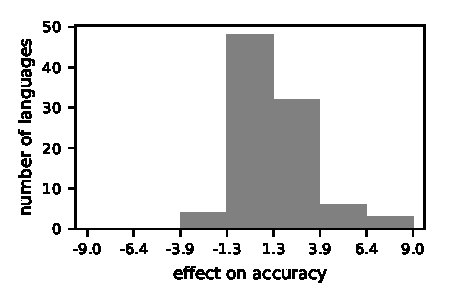
\includegraphics[width=\linewidth]{beamlow}
\caption{Histogramm, welches den Effekt von Beam-Größe 16 im Vergleich zu Größe 1 auf dem Test-Datensatz zeigt (Trainiert auf dem kleinsten Datensatz)}
\label{fig:histBeamLowAcc}
\end{figure}

Auch wenn wir Beam-Decoding für die Einreichung der Daten zum Shared Task nicht verwendet haben, haben wir dennoch im Nachgang Experimente hinsichtlich der Veränderung der Evaluationsergebnisse durchgeführt.
\autoref{fig:histBeamLowAcc} zeigt für wie viele Sprachen ein Unterschied bezüglich der Accuracy durch Beam-Decoding mit einer Größe von 16 im Vergleich zu deaktiviertem Beam-Decoding auftritt.
Knapp die Hälfte der Sprachen zeigt keine oder nur minimale Veränderungen der Accuracy durch Beam-Decoding.
Etwa ein Drittel der Sprachen weist eine leichte Verbesserung der Accuracy zwischen $1,3$ und $3,9$ Prozentpunkten auf.
Während bei einigen Sprachen sogar ein noch stärkerer Anstieg der Accuracy auftritt, zeigen nur wenige Sprachen eine minimale Verschlechterung durch Beam-Decoding.

Über alle Sprachen gemittelt führt der Einsatz von Beam-Decoding mit Größe 16 zu einer Erhöhung der Accuracy von $4\%$.
Ein Binomialtest zur Prüfung, ob es sich ausschließlich um zufällige Erhöhungen handelt, weist im Ergebnis eine Wahrscheinlichkeit von nur $2.4 \times 10^{-10}$ auf.
Daher führt Beam-Decoding zu einem merklichen Anstieg der Accuracy, was auch mit der Intuition übereinstimmt, dass Beam-Decoding bessere oder zumindest gleichstarke Ergebnisse im Vergleich zu \textit{greedy decoding} liefert.

\subsection{Schwachstellen}
\label{sec:schwachstellen}
% Fynn 
Unser System weist mehrere Schwachstellen auf, von denen manche Folgen bewusster Architekturentscheidungen sind, andere jedoch aus einer suboptimalen Implementierung entstanden.

% --- fehlerhafte Umsetzung
So ist die Accuracy unseres Systems bei den Sprachen \lang{Neapolitan} und \lang{Haida} deutlich schlechter im Vergleich zu anderen Systemen und der Baseline wie \autoref{tab:langs_baseline} zeigt.
Die Ursache dafür liegt in der fehlerhaften Nachverarbeitung des String-Transduktors.
Der in \autoref{sec:tuning_evaluation} beschriebene Ausnahmefall beim Korrigieren fehlender \action{EOW}-Ausgaben des neuronalen Netzwerkes tritt für die Sprachen \lang{Neapolitan} und \lang{Haida} oft irrtümlicherweise auf.
Das nachfolgende Beispiel aus dem Test-Datensatz zu \lang{Haida} zeigt, wie unser System in der Ausgabe ein Zeichen \enquote{verschluckt}, da der Transduktor die wiederholte \action{EMIT a} Aktion ignoriert, obwohl das neuronale Netzwerk in diesem Fall eine richtige Vorhersage gemacht hat:
\begin{compactitem}
	\item \texttt{ñíiyä} $\to$ \texttt{ñíiyä'wa\underline{\ }} (Vorhersage)
    \item \texttt{ñíiyä} $\to$ \texttt{ñíiyä'wa\underline{a}} (Ziel)
\end{compactitem}
Solche und ähnliche Fehler treten vereinzelt in den meisten Sprachen auf -- doch in \lang{Neapolitan} und \lang{Haida} sind besonders viele Flexionen betroffen.
Da sich Vorhersage und Ziel-Form jedoch meist nur um ein Zeichen unterscheiden, ist die Levenshtein-Distanz deutlich niedriger als die Accuracy auf den ersten Blick vermuten lässt. So schlagen wir die Baseline auf dem gleichen Datensatz dennoch deutlich hinsichtlich dieser Levenshtein-Distanz.

Die suboptimale Nachverarbeitung im Transduktor hat sich im Rückblick als sehr ärgerlicher Fehler herausgestellt.
Wäre die Nachverarbeitung wie geplant nur dann aktiv geworden, wenn das neuronale Netzwerk gar kein \action{EOW} innerhalb der zulässigen Höchstlänge ausgibt, so hätte die Accuracy unseres Systems im Einklang zu den guten Levenshtein-Ergebnissen eine merkliche Verbesserung gezeigt.

Noch besser wäre es hingegen auf die Nachverarbeitung in Gänze verzichten zu können. Eine Möglichkeit dazu ist die Verbesserung des Trainingsprozesses, indem ein dynamisches Orakel anstelle der statischen Ziel-Sequenz verwendet wird.
Zusätzlich könnte noch globale Normalisierung beim Beam-Decoding eingesetzt werden.
Die Anpassungen am Training des neuronalen Netzwerkes sollten die Probleme der bisherigen Netzwerkausgabe beheben, wodurch auf die fehlerhafte Nachverarbeitung vollständig verzichtet werden kann.

% --- bewusste Architekturentscheidungen
Eine ganz andere Schwachstelle unseres Systems folgt wie bereits erwähnt aus bewusst getroffenen Architekturentscheidungen.
So fällt es unserem System äußerst schwer, Präfixe in Suffixe umzuwandeln und umgekehrt. Das folgende Beispiel aus dem Datensatz für \lang{German} verdeutlicht das Problem:
\begin{compactitem}
	\item \texttt{\underline{ab}stellen} $\to$ \texttt{stellt \underline{\ \ }} (Vorhersage)
    \item \texttt{\underline{ab}stellen} $\to$ \texttt{stellt \underline{ab}} (Ziel)
\end{compactitem}
Das System ist nicht in der Lage, den Präfix \texttt{ab} des Lemmas am Ende der Flexion anzufügen.
Dies ist ein zu erwartendes Verhalten, da unser System die Repräsentationen der Buchstaben monoton nacheinander bearbeitet. Dies geschieht ganz ohne die Möglichkeit frei auf die verschiedenen Stellen des Lemmas zurückzugreifen.
Das neuronale Netzwerk müsste daher die Information des zu Beginn gelesenen Präfixes eines Lemmas so lange im internen Zustand speichern bis dieses am Ende der Flexion wieder auftaucht, da es dem Decoder sonst nicht gestattet ist erneut auf den Anfang des Lemmas zuzugreifen, nachdem das Lemma bereits vollständig durchlaufen wurde.

Um jenes Problem zu lösen, müsste der Decoder mittels \textit{soft-attention} freien Zugriff auf die gesamte Ausgabe des Encoders erhalten. Dadurch wäre jedoch eine erfolgreiche Anwendung der \action{COPY} und \action{PATCH} Aktionen auf dem Lemma nicht mehr gegeben, was zugleich den Kern unseres Systems ausmacht.

\section{Teilnahme am Shared Task und Systembeschreibungs-Paper}
\label{sec:paper}

Der Shared Task als solcher begann am 21. April 2018. An diesem Tag wurden die Trainings- und Development-Daten freigegeben und ein Baseline-System veröffentlicht, das es zu schlagen galt. (Siehe hierzu auch \autoref{sec:baseline}). Neun Tage später wurden die Datensätze in abschließender Version hochgeladen, und ein sogenannter \textit{Feature Freeze} markiert.
Die Teilnahme am Shared Task selbst geschieht hiervon weitgehend unabhängig. So kann nun jeder Teilnehmer der Interesse an dem Thema zeigt, mit der Arbeit beginnen und ein System konzipieren und umsetzen. Die Teilnahme ist an keine verbindliche Anmeldung oder Kostenpauschale gebunden, und die Daten sind prinzipiell frei verfügbar. Darüber hinaus kann sich jeder motivierte Teilnehmer auf der SIGMORPHON Mailing-Liste eintragen, über die wichtige Informationen zum Shared Task kommuniziert werden.

Die Deadline für das Einsenden von finalen Ergebnissen war zunächst für den 20. Juni angesetzt. Wir haben dabei grob angepeilt, diese auch einzuhalten, da der Termin -- eigentlich rein zufällig -- mit unseren Semesterwochen weitestgehend übereinstimmt. Als es zum Ende hin knapp wurde, hat man sich glücklicherweise entschieden, aufgrund eines Problems mit den \textit{surprise languages} noch wenige Tage zu warten und wir hatten somit bis zum 1. August Zeit. Schlussendlich hat es uns das ermöglicht, tatsächlich Ergebnisse einzusenden und zu unserer Überraschung auch nicht mal schlecht abzuschneiden.

Die Beschreibung unseres Systems haben wir mit dem Titel \enquote{Finding the way from ä to a: Sub-character morphological inflection for the SIGMORPHON 2018 Shared Task}\footnote{abrufbar unter \url{https://arxiv.org/abs/1809.05742}} als Paper veröffentlicht.
Pünktlich zur Frist der ersten Abgabe haben wir den Entwurf des Papers anonymisiert am 15. August 2018 eingereicht.
Am 23. August 2018 haben wir die Nachricht bekommen, dass das Paper akzeptiert wurde, sowie das Feedback zweier anonymer Kritiker erhalten.
Dieses Feedback umfasste unter anderem, dass das Paper \enquote{verständlich geschrieben} sei, jedoch mehr Experimente zum Effekt der Patches nötig seien. Man bat uns um weitere Zitate für den Enhancer sowie den Hinweis auf Unicode-NDF-Dekomposition (siehe \autoref{sec:nfd}).
Außerdem haben beide Gutachter das Paper nach bestimmten Kriterien bewertet, siehe Tabelle \ref{tab:review}.
Beide Reviewer haben dabei die gleichen Wertungen abgegeben, nur die \textit{Reviewer Confidence} unterschied sich bei den beiden Gutachtern.
Mit der maximalen Punktzahl wurde die Klarheit des Papers bewertet.
Mit einer Wertung von $3$ wurde der \textit{Impact of Ideas or Results} am schlechtesten bewertet.
Da sich unser System nicht deutlich von anderen System oder bisherigen Ergebnissen absetzen kann, ist diese Wertung nachvollziehbar.
Insgesamt erreichen wir mit $24$ von $30$ Punkten (ausgenommen der \textit{Reviewer Confidence}) $80\%$ der möglichen Gesamtpunktzahl; ein Ergebnis, mit dem wir sehr zufrieden sind.

\begin{table}
\centering
\begin{tabularx}{\linewidth}{Xr}
\toprule
\textbf{Kategorie}            & \textbf{Wertung}  \\
\midrule
Clarity                      & 5            \\
Originality / Innovativeness & 4             \\
Soundness / Correctness      & 4            \\
Meaningful Comparison        & 4             \\
Impact of Ideas or Results   & 3              \\
Recommendation               & 4             \\
\midrule
Total (von 30)               & 24             \\
\midrule
Reviewer Confidence          & 5; 4          \\
\bottomrule
\end{tabularx}
\caption{Wertung der Gutachter auf einer Skala von 1 (schlechteste Wertung) bis 5 (beste Wertung). Beide Gutachter haben die gleichen Werte angegeben, nur die \textit{Reviewer Confidence} unterschied sich.}
\label{tab:review}
\end{table}

\subsection{Poster-Präsentation auf der EMNLP}
\label{sec:paper:emnlp}

Nach dem Erfolg mit unserem Paper zum Workshop angenommen zu werden, stand die Frage im Raum ob man nicht ein Poster auf der EMNLP vorstellt. Dort würden auch alle anderen Teilnehmer ihre Arbeit präsentieren, und es bot sich somit die gute Gelegenheit in den wissenschaftlichen Austausch zu gehen und andere Menschen zu treffen, die sich mit dem selben Shared Task befasst haben.

Nach etwas anfänglicher Skepsis haben wir den Schritt tatsächlich gewagt, und der Arbeitsbereich \texttt{NATS} hat sich dankenswerterweise sogar dazu bereit erklärt, uns finanziell zu unterstützen und die Reisekosten zu erstatten. Mit einem selbst erstellten Poster\footnote{Zum Zeitpunkt der Erstellung dieses Berichts hängt das Poster aktuell in Raum F-432} im Gepäck, welches die Inhalte des Papers erneut zusammenfasst und illustiert, ging es dann am 31. Oktober nach Brüssel. Eine verkleinerte Abbildung findet sich im Anhang als \autoref{app:poster}.

Die Teilnahme am Workshop stand interessierten Zuhörern frei und es kam zu vielen lehrreichen Diskussionen mit anderen Teilnehmern. Ferner waren einige der Organisatoren des Shared Task anwesend, um die Auswertung zu präsentieren. Diese Erfahrungen haben die Projekt-Arbeitsphase fantastisch abgerundet und dafür gesorgt, dass wir jetzt auch in den \textit{Proceedings} der Konferenz zu finden sind.

\section{Hindernisse und was wir daraus gelernt haben}
\label{sec:takeaway}
Wir haben früh angefangen, ein System zu bauen, das erst mal nur \enquote{funktioniert}, und anschließend dieses System ausgebaut und verändert. Dies führte auch dazu, dass die Struktur des Codes zunehmend chaotisch wurde, da wir anfangs mehr Zeit in neue Funktionen investiert haben als in die Pflege des bestehenden Codes. Daher war es zu einem Zeitpunkt nötig, den kompletten Code umzustrukturieren und zu aktualisieren, was wiederum sehr zeitaufwändig war. Für künftige Projekte ist es daher ratsam, früh die Struktur, die man am Ende haben möchte, festzulegen und das Projekt gleich dementsprechend aufzubauen. Dazu gehören insbesondere auch Ordnerstrukturen für Ausgabedateien verschiedenster Art (generierte Daten, Logs, Backups, Evaluation, Grafiken).

Außerdem hatten wir im fortgeschrittenen Stadium des Projekts Probleme, die Logs, die beim Evaluieren der unseres Outputs erstellt wurden, korrekt einzulesen, da wir hier nicht frühzeitig ein einheitliches Format festgesetzt haben. Verschiedene Komponenten haben verschiedene Logs erstellt, die nachträglich vereinheitlicht werden mussten. Dadurch hatten wir später keine Probleme mehr diese Logs zu verarbeiten.

Darüber hinaus haben wir gelernt, wie wichtig Automatisierung ist. Da wir unser System auf mehreren Rechnern verteilt laufen ließen, haben wir Skripte genutzt, die diese aufrufen und die Ergebnisse wieder einsammeln. Weitere Automatisierung hat die Ergebnisse schließlich zusammengeführt und auch die Auswertung sowie Erstellung von Grafiken musste nicht mehr manuell durchgeführt werden.

Eine weitere wichtige Erfahrung ist, wie wichtig Zeitpuffer und Alternativpläne sind, um auf mögliche unvorhergesehene Probleme vorbereitet zu sein. Beispielsweise haben wir unsere finalen Ergebnisse relativ kurz vor Ablauf der ersten Frist inmitten einer Hitzewelle in Hamburg berechnen lassen, was zur Folge hatte, dass die Server, die wir nutzen wollten, wegen eines Ausfalls der Kühlungsanlage abgeschaltet wurden. Wir mussten daher kurzzeitig auf andere, weniger leistungsstarke Server ausweichen:
\foreignquote{english}{\textit{[hummel-users] The sun is killing us (operations down due to cooling system failure)}}

\subsection{Fynn}
Automatisierung ist Trumpf.
Um Verbesserungen schnell evaluieren zu können, ist es essenziell die Ergebnisse aller Trainingsdaten verteilt über mehrere Rechner automatisiert berechnen zu lassen.
Das umfasst das Verteilen der Arbeitspakete, einsammeln der Ausgaben, deren Evaluation und die grafische Aufbereitung, um Effekte klar erkennen zu können.
In diesem Rahmen habe ich meine Shell-Scripting-Fähigkeiten ausgebaut, insbesondere für die zuverlässige Verteilung über mehrere Rechner.

Retrospektiv hatten wir im Team abweichende Erwartungen wie viel wir machen wollen bzw. wie viel Zeit man dafür investiert.
Das hätten wir schon gegebenenfalls während der Gruppenfindung oder zum Start der Bearbeitung des Shared Tasks herausarbeiten sollen.
Dabei half es wenig, dass sich die zeitgleiche, gemeinsame Zusammenarbeit als schwierig gestaltete und effektiv auf die Stunden während der offiziellen Projekt-Zeiten beschränkte.
Es ließen sich keine passenden Zeiten finden, da wir alle nebenbei gearbeitet haben und zusätzlich unterschiedliche Kurse besucht haben.
Daraus resultierte eine relativ strikte Trennung bei der Aufgabenverteilung und reduzierter Wissensaustausch, auch wenn wir versucht haben, die Stunden am Donnerstag vorrangig dafür zu verwenden, den anderen Gruppenmitgliedern das eigene Werk der letzten Woche zu erklären.

Während der Entwicklung unseres Systems habe ich ein tiefgehendes Verständnis neuronaler Netze erlangt, wie es keine Vorlesung geschafft hat -- insbesondere die Verarbeitung dynamischer Sequenzen, Einbau von nicht-Standard Komponenten wie des Transduktors sowie das Einbringen und Ummünzen anderer Ideen (globale Normalisierung, eigene Loss-Funktion, Beam-Decoding etc.) auf das eigene neuronales Netz waren klasse Erfahrungen.
Es hat mir Spaß gemacht, das Netzwerk zu verbessern, um noch mehr Prozentpunkte herauszuholen.
Das erlangte Verständnis hat mir seitdem geholfen neue Paper zu verstehen und wird mir auch Zukunft behilflich sein.

% Auch wenn Python mit PyTorch schnelle Entwicklung und gutes Debugging bietet, wäre für mich eine typisierte und kompilierte Sprache ab einem gewissen Umfang deutlich von Vorteil gewesen -- die optionale Typisierung und Kompilierung bringt bei den eingesetzten Bibliotheken nur wenig.

Ein Paper selbst zu veröffentlichen ist so viel Arbeitet wie erwartet -- aber wahnsinnig cool, wenn das Werk vollbracht ist!
Im Rahmen von Projekt und Seminar habe ich mir viel Wissen über Morphologie in der Computer Linguistik angeeignet.
Dabei habe ich festgestellt, dass Literaturarbeit ewig dauern kann, wenn man Quellen von Quellen liest, man dafür aber immer wieder auf neue Aspekte stößt.

\subsection{Marcel}
Insgesamt war die Projektarbeit sehr lehrreich. Es war sehr verlockend -- und der Verlockung sind wir verfallen -- anfangs \enquote{drauf los zu programmieren}. Wir haben darauf geachtet, einzelne Bausteine zu bauen, die gut miteinander funktionieren und notfalls austauschbar sind, ohne auf zu sehr spezialisierte Schnittstellen angewiesen zu sein. Leider fiel dies zulasten einer geplanten Struktur, die nachträglich zu bauen einige Zeit kostete. Obwohl wir uns schon im Vornherein viele Gedanken über Struktur und Modularität des Systems gemacht haben, hätten wir noch mehr Zeit in diese Planung und die zugehörige Dokumentiert stecken müssen.

Diese Struktur fehlte auch in der Speicherung von Ausgaben und Evaluationen. Dies lag nicht zwingend an mangelndem Willen, sondern vor allem daran, dass die Ausgabe teilweise sehr groß war und es meistens nicht für alle nötig oder möglich war, sie lokal zu speichern. Es fehlte dann aber manchmal die Möglichkeit beispielsweise ein Set an Hyperparametern zu evaluieren, da die Daten einfach gerade nicht verfügbar waren. Das Konstrukt Ausgabe -- Evaluation der Ausgabe -- Evaluation der Evaluationen war meist auf mehrere Rechner verteilt, was nachträgliche Fehlersuche und Erkennung von Zusammenhängen behinderte. Diese Problemstellung ist auf jeden Fall eine, die ich bei weiteren Projekten deutlich stärker beachten und früher planen werde.

Das Projekt erstreckte sich über einen langen Zeitraum, sodass verschiedene Umstände der Gruppenmitglieder aufkamen. Längere geplante wie ungeplante Abwesenheiten etwa durch Urlaub oder Krankheit hatten ihren Einfluss ebenso wie Berufstätigkeit und Semesterferien, sodass einige Gruppenmitglieder streckenweise mehr oder weniger Zeit investieren konnten. Mit diesen Umständen zu planen ist etwas, dessen Wichtigkeit das Projekt gezeigt hat.

Zusätzlich zur Erfahrung in der Projektplanung und Gruppenarbeit hat mir dieses Projekt die behandelten Themen näher gebracht, und gleichzeitig deren Komplexität aufgezeigt. Außerdem konnte ich viel über Python, was ich zuvor nur selten nutzen konnte, Scripting, PyTorch sowie neuronale Netze im Allgemeinen lernen. Darüber hinaus war das Erstellen eines Papers, das offiziell eingereicht und veröffentlicht wird, höchst spannend, aufregend und ungemein zufriedenstellend -- übertroffen nur von dem Gefühl, wenn die Ergebnisse des Systems zum größten Teil nicht nur über den eigenen Erwartungen, sondern auch über der Baseline und dem Durchschnitt der Teilnehmer des Shared Tasks liegen!

\subsection{Gregor}
Ich habe einen sehr tiefen Enblick in die Architektur und den Umgang mit neuronalen Netzen auch im praktischen Anwendungskontext erhalten. Ich fühle mich sicherer bei der Arbeit mit Python-Projekten und insbesondere der PyTorch-Bibliothek. Die Arbeit mit wissenschaftlicher Literatur fiel mir schon vor diesem Projekt nicht schwer, nun habe ich aber eine ganz neue Perspektive dadurch gewonnen selbst einmal solch eine Arbeit veröffentlicht zu haben. Das Publizieren war eine aufregende und bereichernde Erfahrung in meinem Projektverlauf.

Leider habe ich während der Ausarbeitung insbesondere im August immer wieder Rückschläge durch Krankheiten erlebt, vorrangig weil ich empfindlich auf meine Reiseimpfungen reagiert habe. Umso mehr bin ich meinen Mitstreitern in der Projektgruppe dankbar, dass sie trotz meiner vielfachen Abwesenheiten gut weitergearbeitet haben und am Ball geblieben sind. Ich habe mich dann im Gegenzug bemüht, ein aussagekräftiges Poster zu gestalten und durch meine Teilnahme an der EMNLP-Konferenz in Brüssel unsere Ergebnisse auch jenseits der Universität in die Welt hinaus zu tragen.

Mein wichtigstes und größtes Take-Away: Stärkerer Austausch. So sind wir zwar alle drei sehr motiviert an das Projekt gegangen und vom Wissensstand durchaus qualifiziert, aber obgleich die Chemie in der Gruppe gepasst hat, haben wir uns zu wenig zu gemeinsamen Sitzungen getroffen. Immer wieder ist unsere Arbeitsteilung darauf hinausgelaufen, dass jeder Teilnehmer -- mich selbst eingeschlossen -- sein eigenes \enquote{Spezialgebiet} hatte auf dem er sich auskennt, aber dann der Blick in den Code der anderen Gruppenmitglieder nur Verwunderung auslöst und Fragezeichen aufploppen lässt.

TL;DR Es reicht nicht, drei kluge Köpfe die sich gut verstehen zusammen auf eine Aufgabe loszulassen. Vielmehr müssen Teilziele konkreter abgesteckt und Verantwortlichkeiten stärker verteilt werden. Trotzdem bin ich zufrieden und sehr stolz auf das Endergebnis, wobei die Teilnahme an der Konferenz das absolute Highlight war. Danke, NATS!

\section{Ausblick}
\label{sec:future_work}
%\todo[inline]{F: Wir könnten hier wohl auf die Unterüberschriften verzichten}
%\subsection{Mögliche Verbesserungen}

Aufbauend auf dem bisherigen System könnten mehrere Verbesserungen an bestehenden Bestandteilen vorgenommen werden.
Zunächst können die neuen Features, also die Patches und der Enhancer, erweitert werden.

Um Patches weiter zu verbessern, sollte man in erster Linie die Abhängigkeit von einer konkreten Schriftart lösen. Eine mögliche Verbesserung besteht darin, Zeichen in mehreren Fonts zu rendern und auf fehlerhafte Darstellungen zu reagieren. So hat zum Beispiel das typische \enquote{Zeichen unbekannt}-Rechteck den Codepunkt \texttt{U+25A1}; wenn man dieses einmal absichtlich rendert und dann neue Zeichen abgleicht, kann man leicht erkennen welcher Schriftsatz an welcher Stelle Lücken aufweist.
Die zweifelsfrei eleganteste Lösung ist jedoch der Umgang mit dem zuvor erläuterten NFD-Standard des Unicode-Konsortiums. Hier bietet sich die Möglichkeit, fernab jedweder konkreter Schriftarten eine generelle Repräsentation für die Zerlegung von Zeichen zu finden, und diese anhand ihrer Einzelteile in Patch-Klassen einzuordnen. Idealerweise kann man dieses System dann noch mit unserer grafischen Komponente kombinieren, um Redundanzen einzuführen und sich die beiden Systeme gegenseitig ergänzen zu lassen.

Der Enhancer könnte ein besseres Sprachmodell benutzen, um beim Auffüllen der zufällig generierten Worte realistischere Zeichenketten zu erzeugen.
Denkbar wären außerdem eine besondere Behandlung von Prä- und Suffixen, eine bessere Erkennung typischer Silben bzw. N-Gramme sowie das Verhindern von untypischen Buchstabenkombinationen.

% Fynn
Auch am Zusammenspiel von Transduktor und neuronalem Netzwerk können Verbesserungen vorgenommen werden.
So sollte die fehlerhafte Nachverarbeitung im Transduktor durch ein anderes Verfahren ersetzt werden.
In diesem wird die Ausgabe des Netzwerks unverändert übernommen, sofern ein valides Wort mit \action{EOW} als letzte Ausgabe vorliegt.
Nur in dem Fall, wenn das Netzwerk nicht innerhalb der maximalen Ausgabelänge zum Ende kommt, wird in einem Nachverarbeitungsschritt die Netzwerkausgabe beispielweise durch das Lemma ersetzt.
Einen Schritt weiter ginge die Optimierung des neuronalen Netzwerkes, um das Auftreten endloser Ausgaben zu reduzieren bzw. zu unterbinden.
Dazu könnte statt der bisherigen festen Ziel-Sequenz, welche durch den statischen Orakel-Algorithmus erstellt wird, ein dynamisches Orakel eingesetzt werden.
Zusammen mit Beam-Decoding könnte das Training des Netzwerkes dann wie folgt ablaufen:
Für jede weitere Aktion wird je Pfad geprüft, ob diese Aktionskette noch zu einem richtigen Ergebnis führen kann.
Ausschließlich wenn dies nicht der Fall ist, wird ein Trainingsupdate vorgenommen -- ansonsten darf diese Sequenz fortgeführt werden.
Durch ein derartiges Vorgehen sollte das Netzwerk sich besser in beliebigen Zuständen zurechtfinden, wodurch die Robustheit bei ungesehenen Eingaben erhöht wird.

% Letztendlich sollten weitere Parameterkombinationen getestet werden, um die Beste Kombination zu finden. Auch bisher ungetestete Werte für die einzelnen Parameter sollten in Betracht gezogen werden.

%\subsection{Weitere Anwendungsmöglichkeiten}

Darüber hinaus wäre es interessant zu sehen, welche weiteren Möglichkeiten der Anwendung man abseits der Aufgabe erforschen könnte. Beispielsweise könnte man Experimente durchführen um zu beobachten, ob es einen Zugewinn an Genauigkeit gibt, wenn man das System auf mehr als einer Sprache gleichzeitig trainiert. Denkbar wäre es, hier die Sprache als weiteres Feature anzuhängen, sowie entweder nur auf Sprachen derselben Familie zu trainieren, oder Sprachfamilie und gegebenenfalls andere Eigenschaften der Sprache als Features anzugeben. Unter der Annahme, dass Flexionen innerhalb einer Sprachfamilie ähnlich verlaufen, könnten so aus anderen Sprachen korrekte Regeln gelernt und übertragen werden. So könnten Sprachen mit nur geringen Daten trotzdem relativ gut flektiert werden, sofern andere Sprachen derselben Sprachfamilie bekannt sind.

Eine weitere denkbare Anwendung ist die Übersetzung. Dies würde wahrscheinlich größere Anpassungen am System voraussetzen. Übersetzungen innerhalb einer Sprachfamilie sind hier wahrscheinlich erfolgreicher als übergreifend über zwei Familien. Auch mögliche Anwendungen außerhalb der Linguistik, wie beispielsweise chemische Formeln, könnten erforscht werden.

\bibliography{bib}
\bibliographystyle{acl_natbib}

\appendix
\begin{figure*}
	\centering
	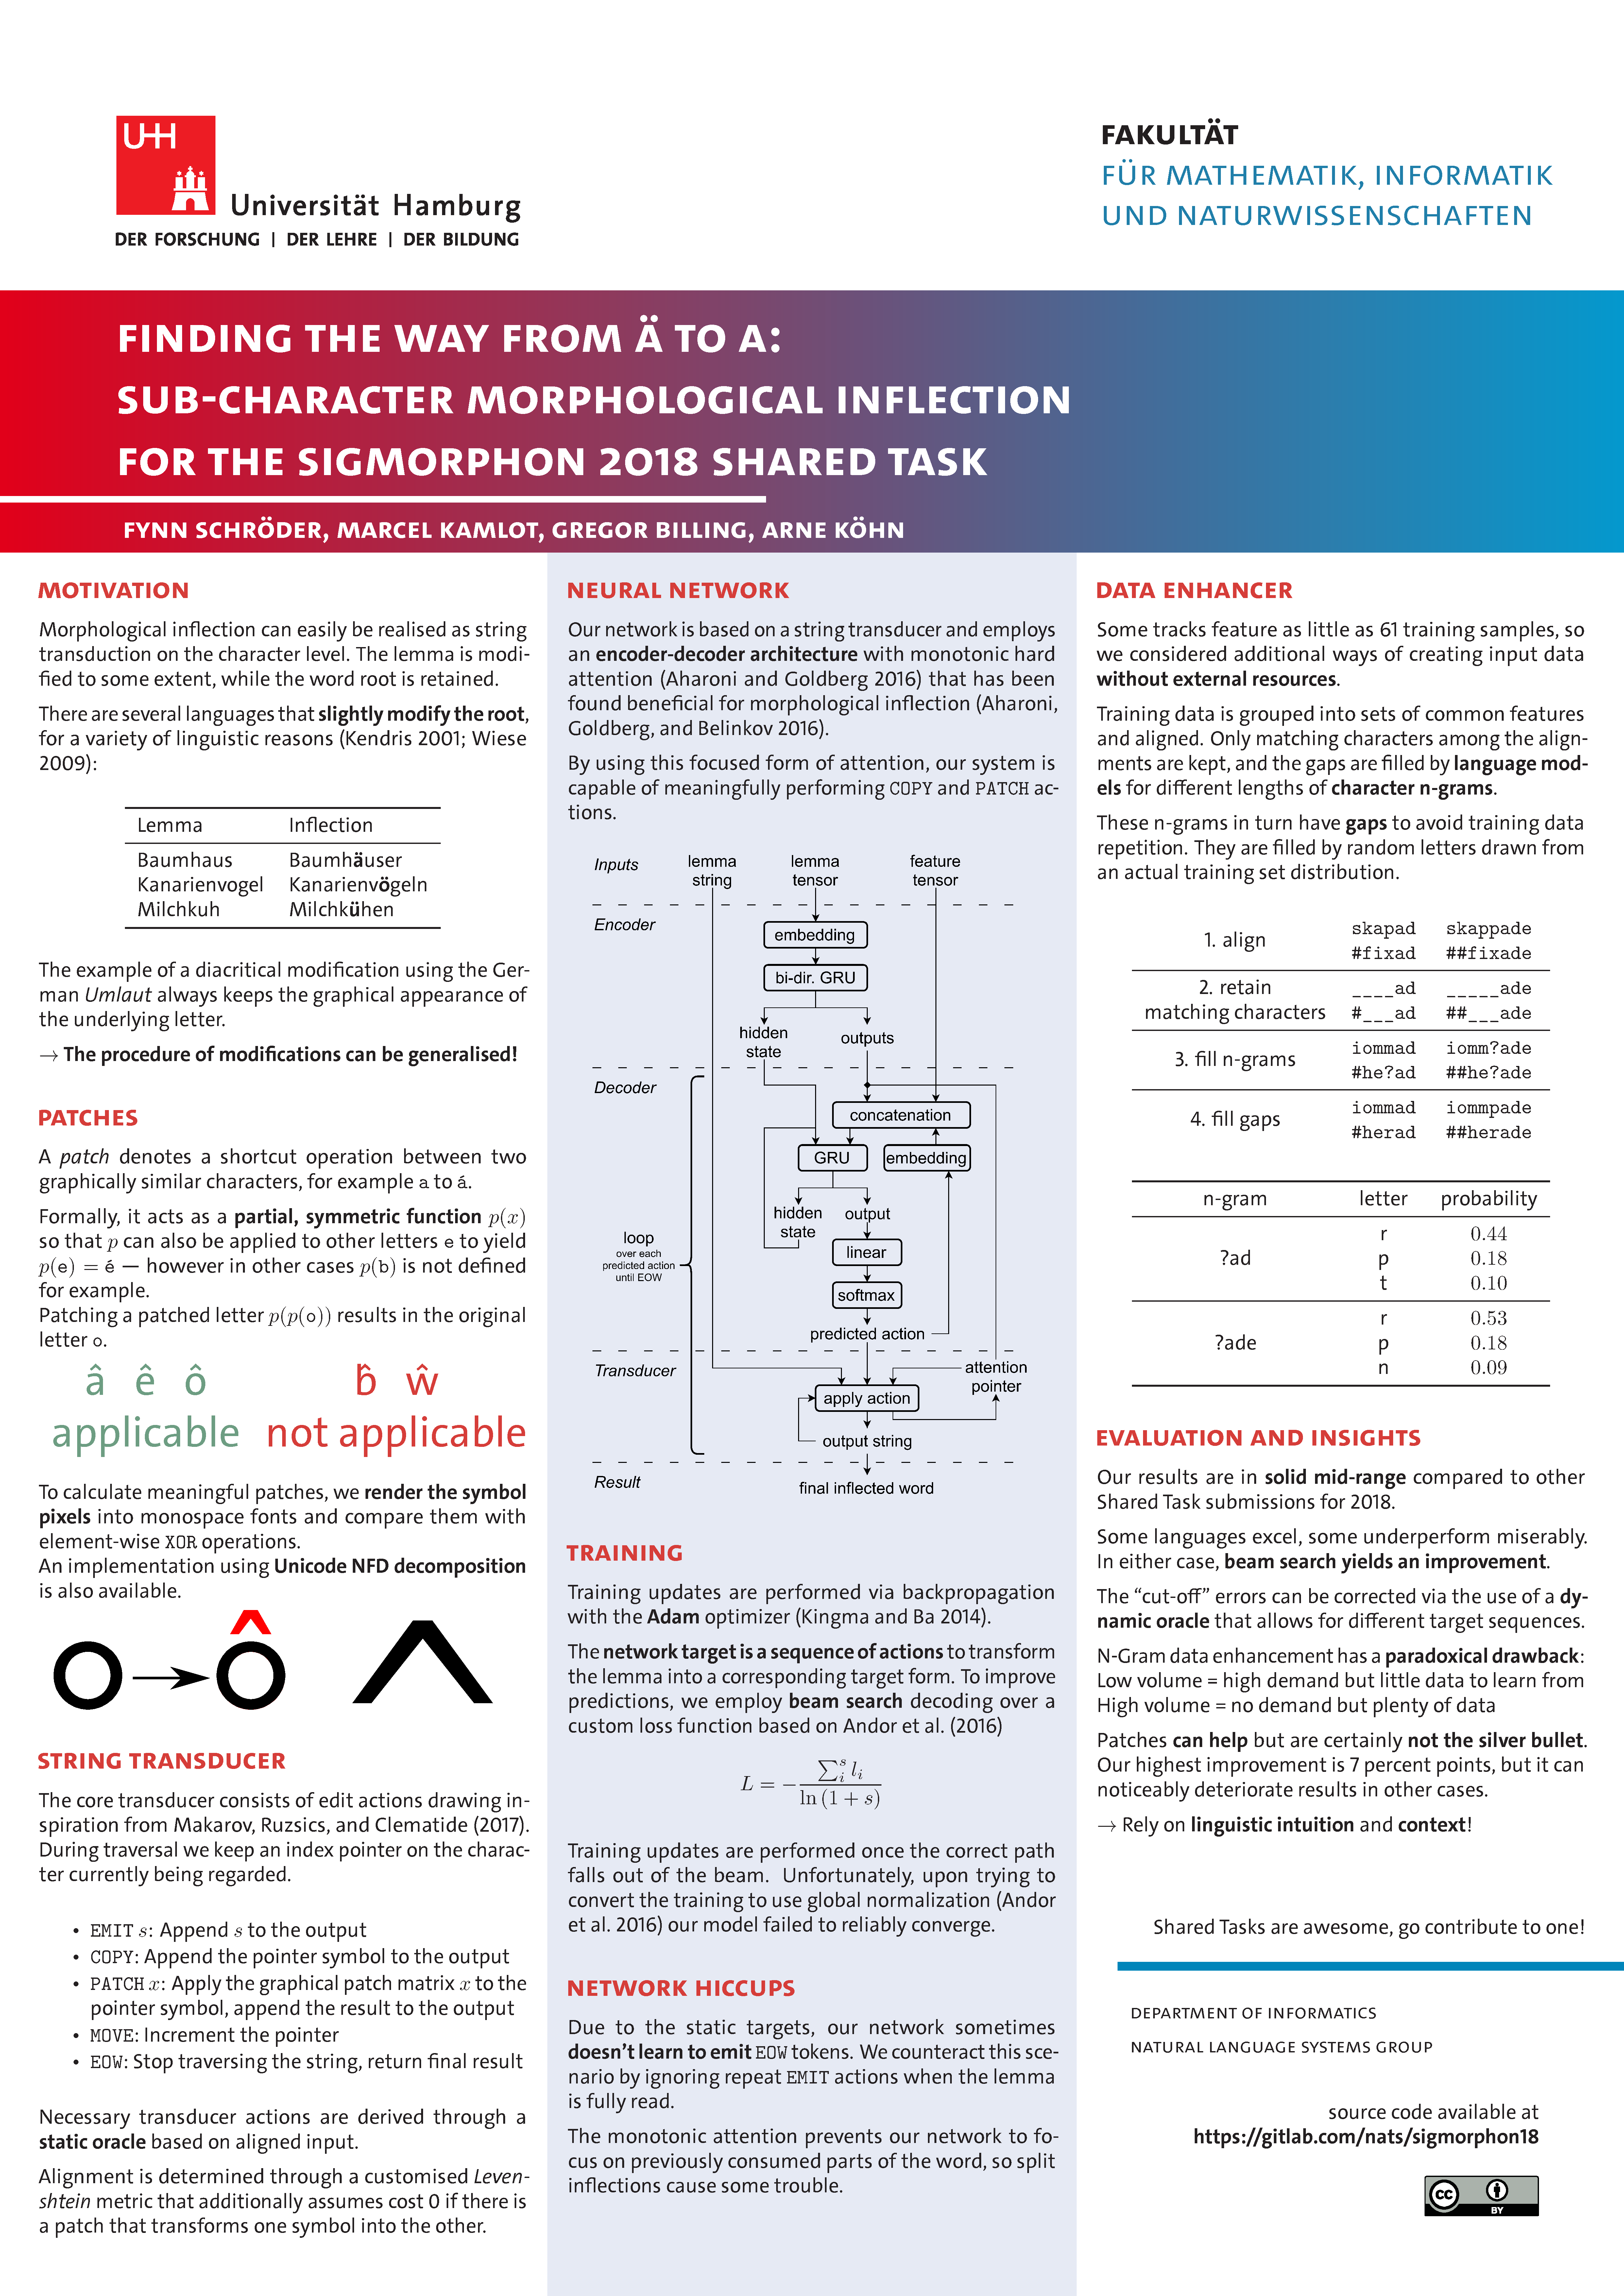
\includegraphics[width=\textwidth]{poster-emnlp.pdf}
	\caption{Das Poster, welches auf dem SIGMORPHON Workshop zur EMNLP-Konferenz 2018 präsentiert wurde}
	\label{app:poster}
\end{figure*}

\end{document}